\documentclass[12pt]{article}
\usepackage{amsmath}
\usepackage{graphicx,psfrag,epsf}
\usepackage{enumerate}
\usepackage{natbib}
\usepackage{amsfonts}
\usepackage{pseudocode}
\usepackage{blkarray}
\usepackage{setspace}
\usepackage{etoolbox}
\newcommand{\blind}{0}



\addtolength{\oddsidemargin}{-.75in}%
\addtolength{\evensidemargin}{-.75in}%
\addtolength{\textwidth}{1.5in}%
\addtolength{\textheight}{1.3in}%
\addtolength{\topmargin}{-.8in}%

\graphicspath{{figures_tables/}}

\begin{document}
\newtoggle{thesis}
\togglefalse{thesis}

%\bibliographystyle{natbib}

\def\spacingset#1{\renewcommand{\baselinestretch}%
{#1}\small\normalsize} \spacingset{1}
  
  
  %%%%%%%%%%%%%%%%%%%%%%%%%%%%%%%%%%%%%%%%%%%%%%%%%%%%%%%%%%%%%%%%%%%%%%%%%%%%%%
    
    \if0\blind
  {
    \title{\bf A GPU accelerated nonparametric shrinkage model for high-dimensional data}
    \author{Eric Mittman\thanks{Department of Statistics, Iowa State University}\\
    and\\
    Jarad Niemi\footnotemark[1]}
      
      
    \maketitle
  } \fi
  
  \if1\blind
  {
    \bigskip
    \bigskip
    \bigskip
    \begin{center}
    {\LARGE\bf A GPU accelerated nonparametric shrinkage model for high-dimensional data}
    \end{center}
    \medskip
  } \fi
  
  \bigskip
  \begin{abstract}
  In high-dimensional settings where traditional shrinkage priors are commonly applied, we consider an alternative nonparametric Bayesian approach based on a Dirichlet process mixture. This highly-flexible approach ``learns" the latent distribution of the random effects to allow for efficient shrinkage toward that distribution. In order to make our approach computationally feasible, we take advantage of the massively parallel architecture of the GPU. We discuss the details of the model and specifics of our implementation of the Gibbs sampler. We use gene expression profiling experiments as a motivating example. Through simulations we study the how the computational time requirements scale with the data. We illustrate our method with a differential expression analysis on a blocked RNA-seq experiment.
  \end{abstract}
  
  \noindent%
  {\it Keywords:}  Bayesian nonparametrics, GPU, high-dimensional, gene expression, Dirichlet process, Gibbs sampling
  
  \spacingset{1.45}
  
  %math macros; figure out where these belong.
\newcommand{\ind}{\stackrel{ind.}{\sim}}
\newcommand{\op}{\operatorname}
\newcommand{\code}{\texttt}

\section{Introduction}
Gene expression profiling studies consider comparisons between experimental groups at many genes on the genome. Typically, because of the large number of comparisons to the number of experimental units, the potential for false discrimination is large. Because of this, there is demand for statistical methods that reduce the number of `false positives' by leveraging information across genes to inform on gene-specific inference.

% Consider the model given by $Y_{gi}|x_i \ind F(\theta_{g}| x_i)$, $g=1,\ldots,G$, $i=1,\ldots,N$ with $G\gg N$ and the quantities of interest are functions of $\theta_g$. In this setting, there is potential benefit to borrow information across group level, $g$, to reduce variance.

A common approach is to model gene-specific parameters as independent, identically distributed according to some probability distribution, $\mathcal{P}$, belonging to a parametric family of distributions. Under this framework, $\mathcal{P}$ can then be estimated allowing for conditional inference, or a prior distribution can be given on its parameters allowing for fully Bayesian inference. While this approach can be useful in practice, the influence of the choice of a particular parametric family can be considerable. This choice is often not reflective of \textit{a priori} information, but rather due to convention or convenience. Here, the choice of a `nonparametric prior', i.e. a prior distribution over a `large' set of probability distributions, allows one to avoid having to make parameteric assumptions about $\mathcal{P}$. 
% The most widely used such prior distribution in the literature of Bayesian nonparametrics is the Dirichlet process (DP).

Much effort has gone into researching methods for analyzing gene expression. Several have been released as R packages \citep{edger2010},\citep{deseq2014}, \citep{voom}. A common feature of these methods is that they use between-gene information to estimate the the  mean-variance relationship nonparametrically. This relationship can be key to acheiving statistical power; it involves both biological and technological sources of variation and varies from dataset to dataset\cite{voom}. Empirically, we have observed structure to be present not only between the mean and variance, but also among regression parameter components (see Fig. \ref{pairs-ind-est}). This suggests that between-gene information is available not only to regulate gene-level assessment of variance, but also the estimated effects themselves. While others used random effects models for individual regression components [\citep{deseq2014},\citep{landau}], they depend on assumptions about the underlying distribution of effects, such as independence, which are contradicted by the data.

\begin{figure}[ht]
\centering
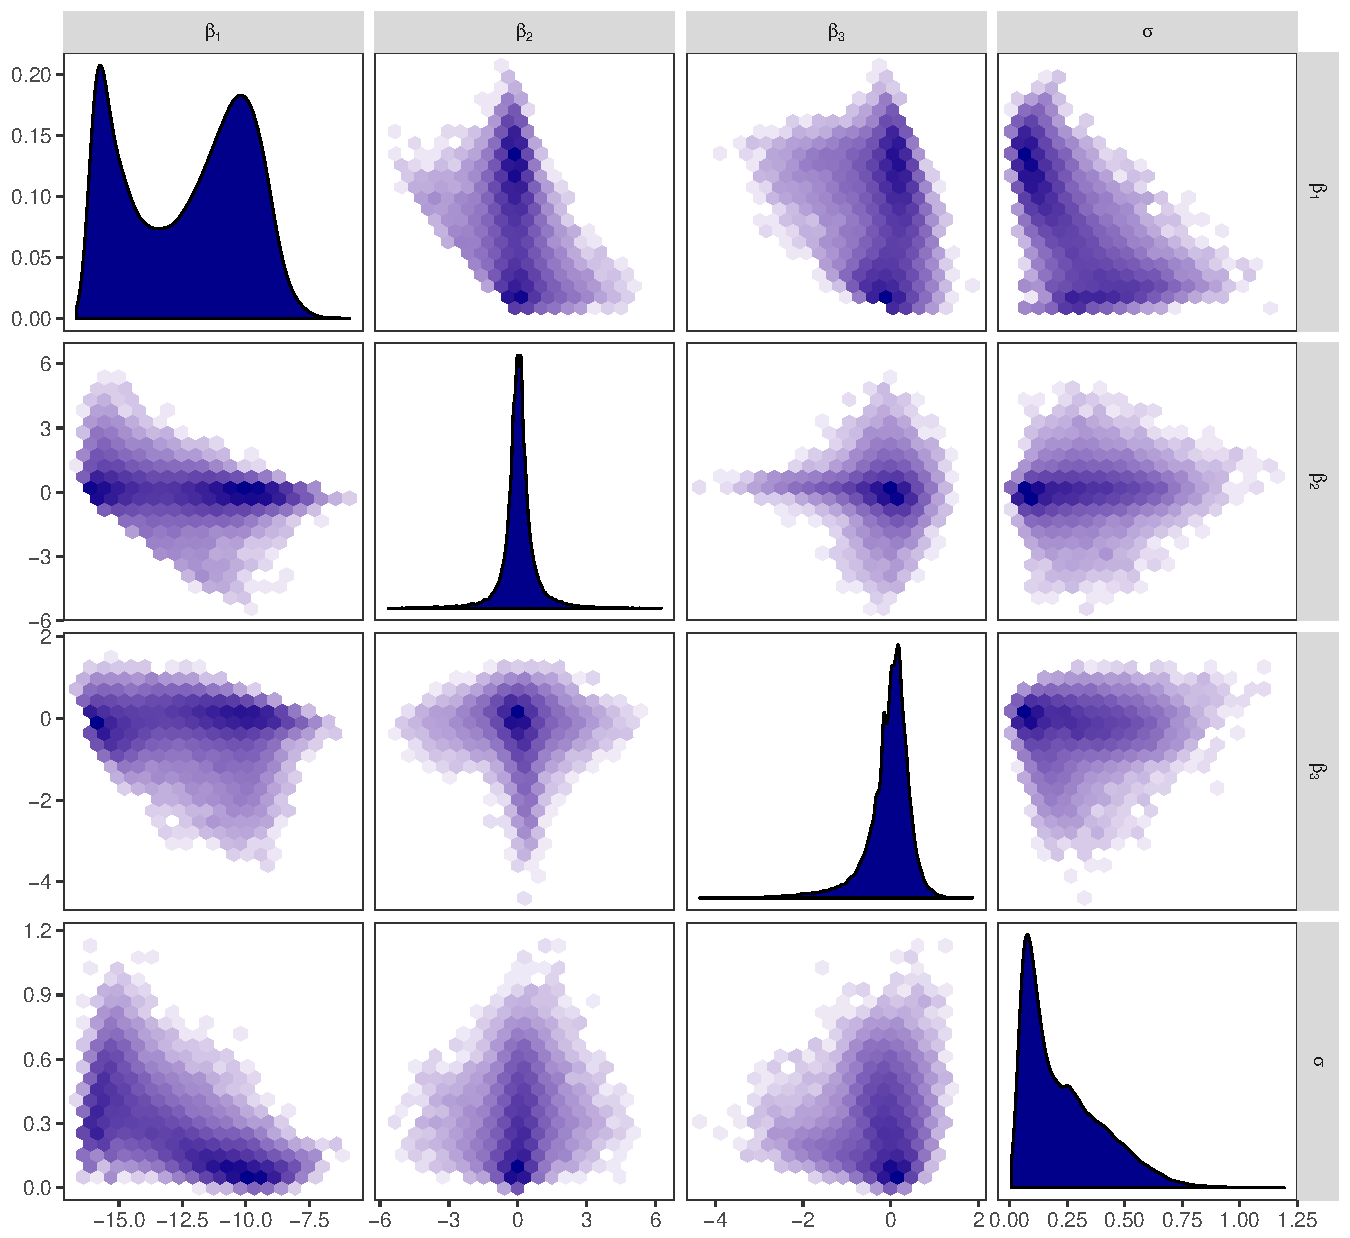
\includegraphics[width=.6\textwidth]{pairs-ind-est-std}
\caption{Bivariate histograms of independent estimates of effects and standard deviation obtained by ordinary least squares for 36,081 genes (data from \cite{paschold}). This example shows that random effects models assuming normality and/or independence may not be suitable for modeling gene expression hierarchically. For more on the data, including definitions of $\beta_1$, $\beta_2$, $\beta_3$, and $\sigma$, see Section \ref{sec:analysis}.}
\label{pairs-ind-est}
\end{figure}

A special case of gene expression profiling concerning two populations is differential gene expression. Because expression is typically modeled on the log scale, the differential expression at a particular gene, termed `log-fold-change', is the parameter of interest. \citet{liu} proposed a semiparametric model treating the log fold change parameters as random effects following an unknown distribution, $\mathcal{P}$, where $\mathcal{P}$ is a random distribution arising from a Dirichlet process. In this paper, we modify and extend the approach taken by \cite{liu} to allow nonparametric inference for a large class of gene profiling experiments. In our method, we use a DP to model jointly the distribution of the $p$-dimensional gene-specific regression coefficient,$\beta_g$, and variance, $\sigma^2_g$.

%The parameters of the DP either chosen, specifying a prior distribution on $\mathcal{P}$, or by placing a prior on these parameters. 
Common practice for Bayesian nonparametric applications is to sample from the joint posterior distribution using a Gibbs sampler. A number of Gibbs sampling algorithms for DP mixture models have been proposed. These can be categorized into two types: `marginal,' where full conditionals are with respect to the joint posterior with the unknown $\mathcal{P}$ integrated out, and `conditional', where $\mathcal{P}$ is also sampled and conditioned on.

When $\mathcal{P}$ is not of particular interest, marginal approaches are often preferable. However, for large $G$, these algorithms are not computationally tractable as they require one-at-a-time updating of the cluster assignment for each $g$ conditioning on all $g'\neq g$. On the other hand, conditional Gibbs methods, which depend on the ``stick-breaking" representation of the DP \citet{sethuraman}, are amenable to parallelism because cluster assignment is conditionally independent given $\mathcal{P}$. \citet{suchard} argued for wider use of graphics processing units (GPUs) by statisticians for computationally demanding, parallelizable tasks to acheive large speed-ups in real time. We provide a brief introduction to computing in the massively parallel context, including some general guidelines that can help in designing implementations that are well-suited for the GPU. We demonstrate that Dirichlet process mixture models for gene expression is feasible in practice by utilizing currently available GPU technology and describe how the implementation was contructed in light of the guidelines.

Section \ref{sec:data} introduces the structure of gene expression profiling data suitable for our method and recommended preprocessing steps. Section \ref{sec:model} presents our model for gene expression, which features a hierarchical model for the gene-specific parameters without parametric assumptions. Next, Section \ref{sec:inference} outlines a procedure for posterior sampling based on the blocked Gibbs sampler of \cite{ishwaran2000}. Section \ref{sec:parallel} introduces concepts related to programming for GPU parallelism and discusses details of two important parallel algorithms. The Gibbs sampler is revisited and GPU implementation details are provided. To investigate the properties of our algorithm, in Section \ref{sec:timing} we discuss a study we conducted to assess the time requirement under variable conditions. Section \ref{sec:analysis} presents an analysis of differential expression data and contrasts our results with both a gene-independent analysis and a mixed-effects analysis assuming a multivariate normal distribution on the random effects. Finally, in Section \ref{sec:discussion} we put our proposed method in context, discuss potential applications and consider future directions for research.
% In summary, to avoid sensitivity to the prior distribution on $\mathcal{P}$, we propose to model it as a truncated Dirichlet process. Advances in computers have seen a rapid increase in the use of Markov Chain Monte Carlo (MCMC) methods for fitting sophisticated statistical models. Because such methods rely on thousands or even millions of simluated draws generated one after another, fast computing is critical to making them computationally feasible. Nonparametric Bayesian methods are no different in this regard, but when the size of the data set gets moderately large, the computational effort required per draw can be enormous as the number of parameters grows with the sample size. Graphics processing units (GPUs) have potential in this area, provided that most of the work can be divided into many parallel tasks which operate on different pieces of memory. By exploiting conditional independence in the model and making use of parallelized algorithms, we demonstrate the feasibility of nonparametric Bayesian modeling in the ``big data" setting of gene expression data.
\section{Data}
\label{sec:data}
We consider gene expression data that can be represented in a tabular format, with rows corresponding to genes and columns to samples (for an abbreviated example, see table \ref{tab:data}). Data meeting this requirement include RNA-seq read counts, but could equally be applied to microarray data. Relevant metadata for the samples include information about groupings, either due to experimental treatment, technical design or natural biological groupings by population. Metadata for the genes themselves, while of great importance to the biologist, are not used by our method.

% latex table generated in R 3.4.1 by xtable 1.8-2 package
% Thu Aug 31 13:00:59 2017
\begin{table}[ht]
\centering
\caption{\small Sample of RNA-seq total read counts from \citep{paschold}. Columns names identify samples, including the genotype and a replicate number, from which we can infer the flow cell that was used for sequencing. Gene annotation information, while available, is not considered as our method does not make use of it.}
\vspace{.2in}
\label{tab:data}
\begin{tabular}{lrrrrrrrr}
  \hline
 & $\mbox{B73}_1$ & $\mbox{B73}_2$ & $\mbox{B73}_3$ & $\mbox{B73}_4$ & $\mbox{Mo17}_1$ & $\mbox{Mo17}_2$ & $\mbox{Mo17}_3$ & $\mbox{Mo17}_4$ \\ 
  \hline
$\mbox{gene}_1$ &   1 &   0 &   0 &   2 &   0 &   1 &   0 &   0 \\ 
$\mbox{gene}_2$ &   3 &   4 &   6 &   0 &   8 &  17 &  18 &  20 \\ 
$\mbox{gene}_3$ & 2323 & 1533 & 1932 & 1945 & 2070 & 1582 & 2196 & 1882 \\ 
$\mbox{gene}_4$ &   2 &   1 &   0 &   2 &   4 &   4 &   5 &   3 \\ 
$\vdots$ &    &    &    &  $\vdots$   &   &   &   &  $\vdots$ \\ 
   \hline
\end{tabular}
\end{table}

\paragraph{Normalization} For various technical reasons, normalization of the table columns (`between-sample' normalization) is needed to adjust for systematic differences arising from technical factors unrelated to the quantities of interest.

For example, in RNA-seq experiments, the total of all read counts (`library size') for a sample will vary, in part, due to differences in sequencing depth. A simple adjustment for library size is to convert total read counts to a relative proportion, such as counts per million (cpm). A criticism of this approach to normalization is that the library size may be driven primarily by a few highly sequenced genes, making this approach too volatile. More robust approaches have been proposed; for further discussion, see \citet{oshlack2010rna}.

\paragraph{Transformation} Because the data are non-negative and variability in expression tends to increase with the overall expression,  gene expression data is typically analyzed on a logarithmic scale, with difference in expression being multiplicative. The large number of zero counts usually present in RNA-seq data, preclude taking logarithms of the raw data. Using a generalized linear modeling approach avoids this problem by specifying a discrete probability model for the counts, while the log-mean expression is modeled as a linear function of the model parameters.

For computational reasons, we assume a normal model for the data after transforming it. First, we compute normalization factor $c_i$ for each column; second, we take logarithms of the data, after adding 1, and apply the normalization on the log scale, .i.e.
$$\mbox{transformed log-count in column }i = \log (\mbox{original count in column }i+1) + \log(c_i)$$. The result after applying these steps to the data in Table \ref{tab:data} are shown in Table \ref{tab:data-transformed}.

% latex table generated in R 3.4.1 by xtable 1.8-2 package
% Thu Aug 31 14:28:27 2017
\begin{table}[ht]
\centering
\caption{\small Same sample of RNA-seq total read counts as in Table \ref{tab:data}, after transformation and normalization. Weighted trimmed mean of M-values normalization was performed using the \texttt{calcNormFactors} function in \texttt{edgeR} \cite{edger2010}.}
\label{tab:data-transformed}
\vspace{.2in}
\begin{tabular}{ccccccccc}
  \hline
 & $\mbox{B73}_1$ & $\mbox{B73}_2$ & $\mbox{B73}_3$ & $\mbox{B73}_4$ & $\mbox{Mo17}_1$ & $\mbox{Mo17}_2$ & $\mbox{Mo17}_3$ & $\mbox{Mo17}_4$ \\ 
  \hline
$\mbox{gene}_1$ & 0.59 & -0.05 & 0.02 & 1.11 & -0.02 & 0.69 & 0.05 & 0.09 \\ 
$\mbox{gene}_2$ & 1.28 & 1.56 & 1.97 & 0.01 & 2.18 & 2.89 & 3.00 & 3.13 \\ 
$\mbox{gene}_3$ & 7.65 & 7.29 & 7.59 & 7.58 & 7.61 & 7.36 & 7.75 & 7.63 \\ 
$\mbox{gene}_4$ & 0.99 & 0.64 & 0.02 & 1.11 & 1.59 & 1.61 & 1.85 & 1.48 \\ 
$\vdots$ &  &  &  & $\vdots$ &  & &  & $\vdots$ \\ 
   \hline
\end{tabular}
\end{table}

\section{Bayesian nonparametric hierarchical regression model}
\label{sec:model}
Let $Y_{gi}$ represent the observed expression (possibly after transformation) for gene $g$, sample $n$. Let $x_{n}^\top$ be the row of the design matrix $X$ corresponding to sample $n$. We will use the upper case letters $G$ and $N$, to denote the number of genes and samples, respectively. In addition, we accommodate possible observation-level weights, $w_{gn}$. For the observed data, we assume the data model
\begin{equation}
Y_{gn} \sim \op{N} \left( x_{n}^\top \beta_g, \frac{\sigma^2_g}{w_{gn}} \right).
\end{equation}
Next, we propose to model jointly

\begin{equation}
\left(\beta_g^\top,\sigma^2_g\right) \ind \mathcal{P},
\end{equation}
where we specify a Dirichlet process on $\mathcal{P}$, i.e.,

\begin{equation}
\mathcal{P} \sim \op{DP}(\alpha \mbox{Q}).
\end{equation}

\iftoggle{thesis}{
The use of this prior, due to \citet{ferguson}, is a distribution over probability distributions, such that for any finite disjoint partition $\{A_i\}_{i>=1}^n$ on $\mathbb{R}^p$, $\mathcal{P}$ is a random measure such that the joint distribution $\left(\mathcal{P}(A_1),\ldots,\mathcal{P}(A_n)\right) \sim \op{Dir}\left(\alpha Q(A_1),\ldots,\alpha Q(A_n)\right).$ The Dirichlet process has two parameters: $Q$, the base measure, represents a prior guess at the distribution. $\alpha$, the concentration parameter expresses the degree to which $\mathcal{P}$ will agree with $Q$ on any set $A$. This follows from the definition given above and known properties of the Dirichlet distribution, i.e., $\op{E}\left(\mathcal{P}(A)\right)=Q(A)$, and $\op{V}\left(\mathcal{P}(A)\right)=\frac{Q(A)(1 - Q(A)}{\alpha + 1}$, showing that $\mathcal{P}(A) \stackrel{p}{\rightarrow} Q(A)$ as $\alpha \rightarrow \infty$ for any set $A$. 
}{}
By modeling $\mathcal{P}$ with a Dirichlet process one can be noninformative about the overall shape of $\mathcal{P}$, allowing for irregular shapes, multimodality, and so forth. An argument can be made that by incorporating our uncertainty about these features of the distribution is required for coherent interpretation of the posterior distribution \citep{walker2010bayesian}. For more information about the properties of the DP, see \cite{ferguson}.

As shown by \citet{sethuraman}, it follows from the definition of the Dirichlet process that $\mathcal{P}$ is almost surely discrete and realizations of $\mathcal{P}$ can be produced by the following stick-breaking construction:

Let 
\begin{equation}
\mathcal{P} =\sum_{k=1}^\infty \pi_k \delta_{\left(\tilde{\beta}_k^\top ,\tilde{\sigma}^2_k\right)}.
\end{equation}
Here $\delta_{(.)}$ is the Dirac delta function. Note that although almost sure discreteness is a property applicable to ``draws'' from a DP, the posterior for $\mathcal{P}$ is in fact a mixture of DP \citep{antoniak}. An implication of discretness can be thought of as a ``bet on sparsity"; that there are actually a finite (but unspecified) number of unique values that $(\beta_g^\top,\sigma^2_g)$ can take.  
 The ``atoms" distributed according to $Q$, specified by the product measure

\begin{equation}
\tilde{\beta}_k \sim \op{N}(m_\beta, C_\beta),\quad \tilde{\sigma}^2_k \sim \op{IG}(a_{\sigma^2}, b_{\sigma^2}).
\end{equation}

``$\op{IG}(a,b)$" refers to the inverse gamma distribution which we parameterize by shape and scale parameters, $a$ and $b$ with density given by
\begin{equation*}
p(x|a,b) = \frac{b^a}{\Gamma(a)}x^{a+1}e^{-b/x}.
\end{equation*}


The mixture weights, $\pi_k$,  follow a stick-breaking process \cite{sethuraman}. Using the reparameterization,

\begin{equation}
\nu_k = \frac{\pi_k}{1 - \sum_{l=1}^{k-1} \pi_l},
\end{equation}

$\nu_k$ representing a proportion of the total probability remaining after $k-1$ breaks. For the stick-breaking construction of the DP, the $\nu_k$ are modeled by:
\begin{equation}
\nu_k \ind \op{Beta}(1, \alpha).
\end{equation}

This assumption induces a stochastically decreasing ordering of the weights. Additionally, note that $\sum_{k=1}^K \pi_k \stackrel{p}{\rightarrow} 1$ as $K\rightarrow \infty$. 



\section{Model inference}
\label{sec:inference}
In order to make inference with this model, we invoke Bayes' theorem, which requires the choice of prior distributions to complete a full probability model.

We choose values of $m_\beta,\,C_\beta,\,a_{\sigma^2},\,b_{\sigma^2}$ to put mass on reasonable values of $\left(\beta_g^\top,\sigma^2_g\right)$. This can be though of as an empirical Bayes approach. Alternatively, one could specify priors on these parameters, adding another hierarchy to the model. In any case, choosing Q to be diffuse can be overly informative and lead to only few large $\pi_k$ accounting for most of the total probability in the mixture, $\mathcal{P}$ \citep{gelman-book}.

The parameter $\alpha$ plays an important role in the model, since it helps to determine how quickly the successive elements of $\pi$ decay, i.e. the number of clusters selected by the model. For computational convenience, we choose the conditionally conjugate prior

\begin{figure}
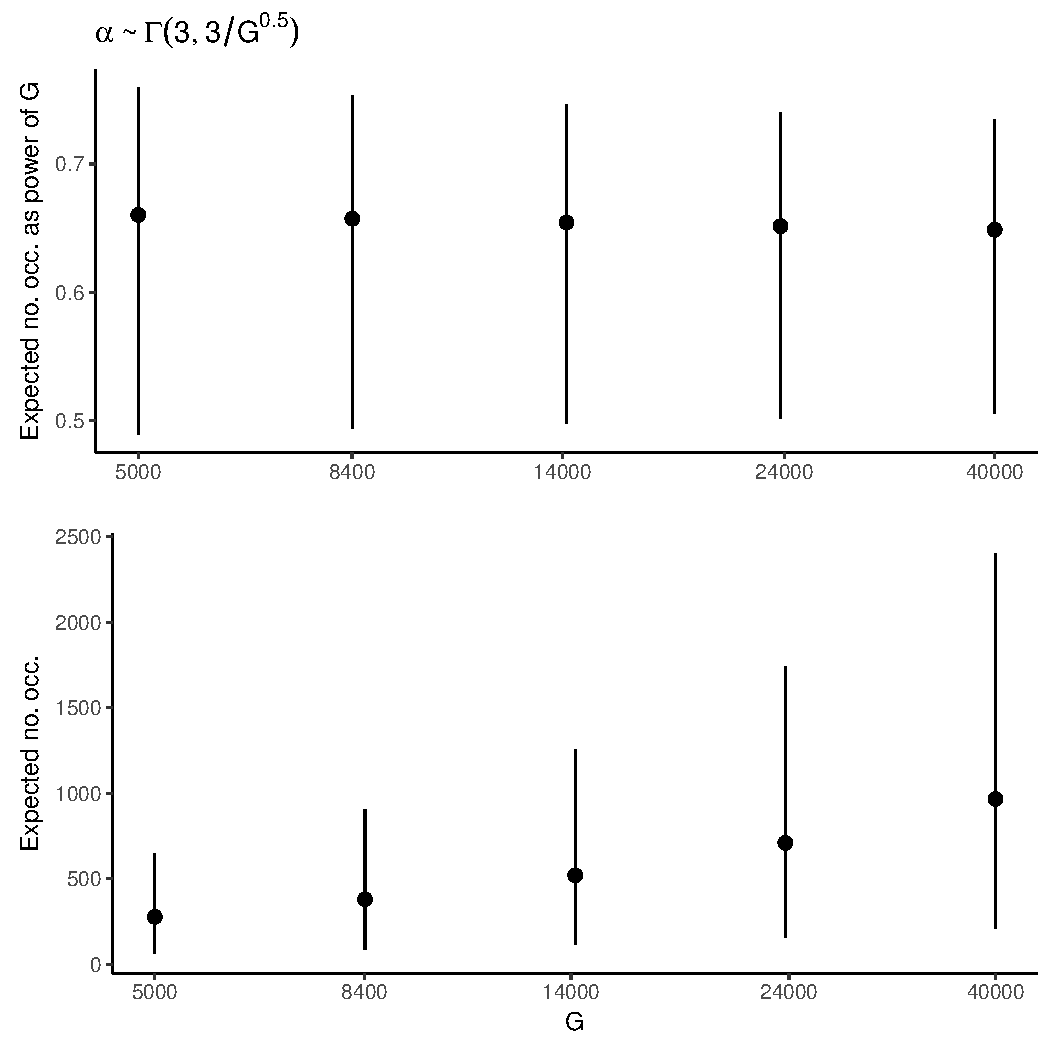
\includegraphics[width=.5\textwidth]{alphaprior}
\caption{The number of clusters determined by the model is influenced by the parameter $\alpha$, whose value determines the expected number of clusters prior to seeing the data. The figures above demonstrate the prior distribution of the prior expected number of clusters, $\op{E}(K_{occ})$ for datasets with various number of genes, $G$.}
\label{alphaprior}
\end{figure}

\begin{equation}
\alpha \sim \op{Ga}(a_\alpha,b_\alpha).
\end{equation}

This prior can be selected to express an a priori belief on the number of clusters, $K_{occ}$, in the data. \citet{escobar1994} give expression for the expected value of $K_{occ}$ given $\alpha$ and $G$ as,
\begin{equation}
\op{E}(K_{occ})=\sum_{g=1}^{G} \frac{\alpha}{\alpha + g - 1}.
\end{equation}
In that paper, the authors use a table of values derived from this formula to defend their proposal for a prior over values of $\alpha$ ranging from $G^{-1}$ to $G^{2}$, which admits values of $\op{E}(K_{occ})$ anywhere from 1 to $G$. Due to computational limitations (we require $K_{occ} \ll G$), and our prior belief, based on scientific evidence, that there are more than just a few clusters, we choose $a_\alpha=3$ and $b_\alpha=\frac{3}{G^{.5}}$ to express a prior that $\op{E}(K_{occ})$ is probably between $G^{.5}$ and $G^{.75}$ (see figure \ref{alphaprior}).

\subsection{Data augmentation and the TDP}
\label{subsec:reparam}

\begin{figure}
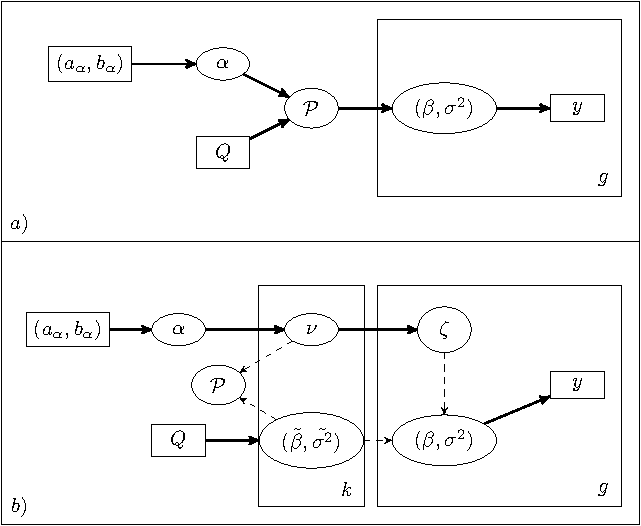
\includegraphics[width=.8\textwidth]{my_dag}
\caption{Directed acyclical graphs of the Bayesian nonparametric hierarchical regression model. Panel $(b)$ introduces latent allocation parameters, $\zeta_g$, which decouple the process which partitions the data into clusters from the distribution which provides the unique values, $(\tilde{\beta_k},\tilde{\sigma}_k^2)$ of the cluster parameters. Solid lines indicate distributional dependency, dashed lines indicate deterministic functional relationships.}
\label{dag}
\end{figure}

Panels (a) and (b) in Figure \ref{dag} shows a graphical two representations of the model. As explained in \cite{neal2000}, while sampling methods based on $a)$ exist, it is more efficient to decouple the process partitioning the $(\beta_g,\sigma_g)$ into clusters from the process providing the unique values, $Q$. This is done by introducing a latent variable, $\zeta_g$, taking values on the positive integers with the discrete distribution given by $Pr(\zeta_g=k)=\pi_k$. These latent variables generate a random partition of the `genes' into groups, with $(\beta_g,\sigma^2_g)=(\tilde{\beta}_k,\tilde{\sigma^2}_k)$ for all $g$ where $\zeta_g=k$. The expanded form of the model is shown in $b)$.

Our Gibbs sampler is based on that proposed by \citet{ishwaran2000}. In contrast to prior approaches to MCMC, detailed in \citet{neal2000}, which can be classified as ``marginal" methods, Ishwaran and Zarepour presented their ``blocked" Gibbs sampler which allows approximate inference for DPM models. Unlike the marginal Gibbs samplers, which update the cluster allocation for each
`gene', conditional on all other allocations, the blocked sampler jointly updates all cluster allocations independently. Being able to do so is advantageous when $G$ is large, since it becomes possible to do a large portion of the necessary computation using many concurrent processes. As we can see from Figure \ref{dag}, $\zeta_g$ are conditionally independent given $\mathcal{P}$. This is problematic since $\mathcal{P}=\sum_{k=1}^\infty \pi_k \delta_{(\beta_k,\sigma^2_k)}$ is an infinite mixture. \cite{ishwaran2001} showed that, due to the stochastic ordering of the $\pi_k$, $\mathcal{P}$ can be well-approximated by $\mathcal{P}_K=\sum_{k=1}^K \pi^*_k \delta_{(\beta_k,\sigma^2_k)}$, letting $\pi_k^*=\pi_k$ for $k<K$ and $\pi_K^* = 1-\sum_{k=1}^{K-1} \pi_k$. The authors provide an approximate lower bound to the $L_1$ distance between $\mathcal{P}_K$ and $\mathcal{P}$ as a function of $G$, $K$ and $\alpha$ and argue that because the bound decreases exponentially with $K$, it should be possible in practice to use a hierarchical model based on $\mathcal{P}_K$ that is virtually indistinguishable from one based on $\mathcal{P}$.

Applying this truncation in our model is acheived by setting $\nu_K=1$. We then have

\begin{equation*}
\zeta_g \sim \op{Cat}_K(\pi) = \sum_{k=1}^K \pi_k \delta_{k}, \mbox{ i.e. } Pr(\zeta_g=k)=\pi_k.
\end{equation*}


% In general, scientific questions will be restricted to those which can be formulated as sets of linear inequalities in $\beta_g$. 
%question: in genes with small counts, does this assumption lead to multimodality in posterior for beta_g?

\subsection{Posterior distribution}
\label{subsec:posterior}


Applying Bayes' theorem, the posterior distribution, up to a constant, is
\begin{equation*}
p(\beta,\sigma^2,\mathcal{P},\alpha|y) = p(\zeta, \tilde{\beta},\tilde{\sigma^2},\nu,\alpha | y) \propto p(y|\tilde{\beta},\tilde{\sigma^2},\zeta) p(\zeta|\nu) p(\nu|\alpha)p(\tilde{\beta},\tilde{\sigma^2})
\end{equation*}
\begin{equation*}
= \prod_{g=1}^G \left\{ \op{N}(y_g;\,\beta_{\zeta_g},\sigma^2_{\zeta_g})\; \op{Cat}(\zeta_g;\, \pi(\nu)) \right\} \prod_{k=1}^K \left\{ \op{Be}(\nu_k;\, 1, \alpha)\; \op{N}(\tilde{\beta_k};\,m_\beta, C_\beta)\;\op{IG}(\tilde{\sigma}^2_k;\,a_{\sigma^2},b_{\sigma^2})\right\} \op{Ga}(\alpha;a_\alpha,b_\alpha)
\end{equation*}
The first equality follows from the  invariance to reparameterization of the posterior distribution, and the last equality follows from the product rule of conditionally independent random variables.

\subsection{Full conditionals}
\label{subsec:full-cond}
Our blocked Gibbs sampler is constructed as follows:
\paragraph{Step 1:}
Both the allocation parameters, $\zeta_g$ and the DP concentration parameter, $\alpha$, are conditionally independent given $\pi, \beta, \sigma^2$ and the full conditional distribution is given by

\begin{equation}
p(\zeta, \alpha|\cdot) \propto \prod_{g=1}^G \left[ \op{N}(y_g;\,\beta_{\zeta_g},\sigma^2_{\zeta_g}W_g)\; \op{Cat}(\zeta_g;\, \pi(\nu)) \right] \prod_{k=1}^K \left[ \op{Be}(\nu_k;\, 1, \alpha)\; \op{Ga}(\alpha;a_\alpha,b_\alpha)\right],
\end{equation}
with conditional independence being implied by the product rule. For $\zeta$ we get
\begin{equation}
\label{zetafull}
p(\zeta|\cdot) = \op{Cat}_K(\hat{\pi}_k), \mbox{ with}
\end{equation}
\begin{equation*}
\hat{\pi}_k \propto \pi_k \op{N}(y_g;X\tilde{\beta}_k,\tilde{\sigma}_k^2 W_g).
\end{equation*}

We see that $\alpha$ depends only on $\nu$:
\begin{equation}
    p(\alpha|\cdot) \propto \prod_{k=1}^{K-1} \op{Be}(\nu_k;1, \alpha) \; \op{Ga}(\alpha;a_\alpha,b_\alpha)
\propto \alpha^{(K-1) + a_\alpha - 1} \left(\prod_{k=1}^{K-1} (1-\nu_k)\right)^\alpha e^{-b_\alpha \alpha} 
  \end{equation}
  \begin{equation*}
    = \alpha^{(K-1) + a_\alpha - 1} e^{-(-\log \pi_K + b_\alpha) \alpha}
  \end{equation*}
  \begin{equation*}
    \implies p(\alpha|\cdot) = \op{Ga}(K + a_\alpha - 1, -\log \pi_K + b_\alpha)
  \end{equation*}



The full conditionals for $\tilde{\beta}_k$ and $\tilde{\sigma}^2_k$ are straightforward, due to conjugacy. However, for a given $k$, the full conditional for $\tilde{\beta}_k$ depends on $\tilde{\sigma}^2_k$, and visa versa.

\paragraph{Step 2:} 
The full conditional for cluster location, $\tilde{\beta}_k$:
    \begin{equation}
      p(\tilde{\beta}_k|\cdot) \propto \prod_{g:\zeta_g=k} \op{N}(y_g;\,X\tilde{\beta}_k, \sigma^2_gW^{-1}_g)\,\op{N}(\tilde{\beta}_k; m, C)
    \end{equation}
    \begin{equation*}
      \implies p(\tilde{\beta}_k|\cdot) = \op{N}(\tilde{\beta}_k; \hat{m}_k,\, \hat{C}_k),
    \end{equation*}
    \begin{equation*}
    \mbox{ where }\hat{C}_k= \left( \sigma^{-2}_g\sum_{g:\zeta_g=k}
      X^\top W_g X + C^{-1} \right)^{-1}, \mbox{ and
    }\hat{m}_k=\hat{C}_k \left(\sum_{g:\zeta_g=k} X^\top W_g y_g +
      C^{-1}m \right).
    \end{equation*}
\paragraph{Step 3:} The full conditional for cluster variance, $\tilde{\sigma}_k^2$, is:
    \begin{equation}
      p(\tilde{\sigma}_k^2|\cdot) \propto \prod_{g:\zeta_g=k}
      \op{N}(y_g;\,X\tilde{\beta}_k, \sigma^2_gW^{-1}_g)
      \op{IG}(\tilde{\sigma}_k^2; a_{\sigma^2},b_{\sigma^2})
    \end{equation}
    \begin{equation*}
      \implies p(\tilde{\sigma}_k^2|\cdot) = \op{IG}(\hat{a}_k,\hat{b}_k), 
    \end{equation*}
    \begin{equation*}
      \mbox{ where }\hat{a}_k = a_{\sigma^2} + \frac{NM_k}{2},\mbox{ and }\hat{b}_k= b_{\sigma^2} + \sum_{g:\zeta_g=k}y_g^\top W_g y_g -2 \beta_g^\top X^\top W_g y_g  +\beta_g^\top X^\top W_g X \beta_g
    \end{equation*}

    Here $M_k$ is the number of $g$ for which $\zeta_g = k$. 
\paragraph{Step 4:} The full conditional for $\nu_k,\,k=1,\ldots,K-1$ depends only on $M_k(\zeta)$. The full conditional is:

  \begin{equation}
    p(\nu_k) \propto \prod_{l \ge k} \prod_{g:\zeta_g=k} \pi_k \; \op{Be}(\nu_k; 1, \alpha) \propto \nu_k^{M_k + 1}(1-\nu_k)^{\sum_{l > k} M_l + \alpha} 
  \end{equation}
  \begin{equation*}
    \implies p(\nu_k)=\op{Be}(M_k + 1, \sum_{l>k}M_l + \alpha)
  \end{equation*}

\section{Computation on the GPU}
\label{sec:parallel}
\subsection{General Remarks}
Modern GPUs offer hundreds or thousands of cores that can provide concurrent excecution. Compared with multi-core CPUs, which typically boast 16 or fewer processors, this suggests a large benefit to using GPUs to exploit parallelism. While these benefits are becoming more widely recognized and gaining visibility through some large software projects such as Tensorflow, as with any technology there limitations, trade-offs and can be additional complications. We now direct attention to some differences in implementation, compared to traditional CPU programming, that are required when porting code to a GPU platform.

GPUs are usually subservient to a host CPU: the executing program is run on a CPU which turns over control periodically to the GPU to run specific tasks. These tasks, or ``kernels", follow the single instruction, multiple data (SIMD) paradigm. Each core on the GPU is assigned to work on a specific chunk of memory, but all cores execute the same program. Each instance of the program is called a ``thread". It is desirable to avoid branching logic in kernels, in part because the GPU cores are relatively slow, so branching can easily lead to high latency. The best results are obtained by having all threads proceed in lockstep.

The GPU has its own memory system. Because copying memory from host (CPU) to device (GPU) and visa versa is slow, if possible, data input should be copied only once from the host CPU to GPU memory and when the task is completed, it should be copied once back only once to the CPU.

When programming for the CPU, memory accesses tend to be fast. On the GPU, while the thread local memory is fast, its size is limited, and reading and writing from global memory is slow. Therefore, kernels need to limit both reads and memory allocation, or else the potential gain in speed due to parallelism will be lost due to memory bottlenecks.

Threads are themselves organized into ``warps". When data is read from global memory, it reads not one address at a time, but in chunks to minimize overhead costs. To take advantage of this, consecutively indexed threads should use data from memory at consecutive addresses. When this happens, the reads are ``coalesced". If consecutive threads access addresses that are distant to one another, reads are not coalesced, which will make memory transfer inefficient, hence the program will tend to be slow.

\subsection{Routines}
\label{sec:routines}
\subsubsection{Reductions}
\label{subsec:reduce}
On the GPU, individual processors are slow, and asynchronous tasks can result in many idle threads. In order to achieve speed-ups, algorithms must exploit parallelism and must do so in a way that respects the limitations of the hardware. A basic example is reduction. Given some data in memory, $x_1, x_2, \ldots, x_n$, and an \textit{associative} operator $+$, the problem is to compute $s_n=x_1 + x_2 + \ldots + x_n$. 

\begin{pseudocode}[ruled]{Reduce}{a}
\label{upsweep}
\COMMENT{Parallel reduction of $n=2^D$ elements (upsweep step of cumulative `sum`).}\\
\FOR d \GETS 1 \TO D \DO \BEGIN
  \FOR i \GETS 1 \TO n \mbox{ in parallel }\DO \BEGIN
    \IF i \mbox{ mod } 2^d \DO \BEGIN
    a[i] \GETS a[i-2^{d-1}] + a[i];\\
    \END \END \END
\RETURN{a}
\end{pseudocode}

To see why the reduce algorithm works, we consider using reduce to compute a sum of $2^D$ elements. Let $a$ an array of size $n=2^D$ ($a=(a_1,\ldots,a_n)$) containing values $v_1,\ldots,v_n$. Define $z(i)=\op{argmax}_{d\ge 0}\{i \mod_{2^d} =0\}$; or, alternatively, the number of trailing zeros when $i$ is written in binary. At the end of iteration $d$ of the outer loop, $a_{i},\,i$ in $\{j\cdot 2^d: 1 \le j \le 2^{D-d}\}$ contains the sum, $s_{i}-s_{i-2^d}$, allowing the target, $s_n$, to be computed by $\sum_{j=1}^{2^{D-d}}(s_{j\cdot 2^d}-s_{(j-1)\cdot 2^d})$. In the last iteration, the target is computed simply by adding the partial results in $a_{2^{D-1}}$ and $a_{2^{D}}$. We note here that, upon completion of the routine, $a_i$ contains a partial sum which depends on $z(i)$, namely $s_i - s_{i-2^{z(i)}}$.

Assuming no constraint on the number of processors, algorithm \ref{upsweep} illustrates good GPU programming strategies. In the first iteration of the outer loop, the inner loop keeps a maximal number of threads busy with identical tasks, requiring similar and parallel memory accesses, two reads and one write. While half of these threads become idle in subsequent loops, the active threads always write to the same place. In practice, since device memory is not flat, as was discussed in the previous subsection, an optimal implementation would make use of shared memory after the first read. Reading and writing from shared memory is much faster than from global memory and is accessible to all threads in a block.

% CUDA users who want to take advantage of GPU parallelism without concerning themselves with the optimization should be aware of the Thrust library \cite{thrust}. Thrust is based on the C++ Standard Template Library and provides both containers for handling allocation and deallocation of device memory as well as generic algorithms, such as \code{thrust::reduce}.


%\caption{Parallel reduction of $n=2^d$ elements (upsweep step of scan). Upon return, total is stored in $a[n]$.}

\subsubsection{Cumulative (prefix) sums}
\citet{blelloch1990} described a general algorithm for computing $x_1,
x_1 \oplus x_2, \ldots, x_1 \oplus \ldots \oplus x_n$. This kind of routine is a generalization of a cumulative sum and is used in various ways in our MCMC algorithm. For example, the calculation of cumulative probabilities to sample from categorical distributions in step 1 computes the cumulative sum on the log scale for numerical stability, i.e. $\oplus=\log(e^{x_1}+e^{x_2})$.

\begin{pseudocode}[ruled]{CumulativeSum}{a}
\label{downsweep}
\COMMENT{Parallel cumulative (prefix) sum of $n=2^D$ elements.}\\
a \GETS \CALL{Reduce}{a}\\
a[n] \GETS 0\\
\FOR d \GETS D-1 \TO 0 \DO \BEGIN
  \FOR i \GETS 1 \TO n \mbox{ in parallel }\DO \BEGIN
    \IF i \mbox{ mod } 2^{d+1} = 0 \DO \BEGIN
    tmp \GETS a[j-2^{d}];\\
    a[i-2^{d}] \GETS a[i];\\
    a[i] \GETS tmp \oplus a[i];
    \END \END \END
\RETURN{a}
\end{pseudocode}

A serial version of this algorithm, $z_1 = x_1,\;z_2 = z_1 \oplus x_2,\dots$, is ill-suited to the GPU. Blelloch showed that there is an efficient parallel alternative. The simplest case is for an array with $2^d$ elements and $2^{d-1}$ processors. The algorithm is composed of two steps: a parallel reduction (referred to in \cite{blelloch1990} as``upsweep"; Algorithm \ref{upsweep}), followed by a ``downsweep" (Algorithm \ref{downsweep}. Given an input array $a$, an upsweep followed by a downsweep modifies the array $a$, defined above, so that $a_i$ contains $s_{i-1}=\sum_{j=0}^{i-1}v_j$, where $v_0$ is the identity element.

The downsweep works with the partial results in memory after the upsweep. Picking up the example of the last subsection, define $b_{i,D}b_{i,D-1}\cdots b_{i,1}b_{i,0}$ to be the binary representation of the integer $i$. For example, if $D=4$, $i=11=01011_{2}$, with $b_{i,4}=0,\, b_{i,3}=1,\,b_{i,2}=0,\,b_{i,1}=1$ and $b_{i,0}=1$. For each $b_{i,d}=1$ in $b_i$, there is a partial sum of $2^d$ values produced in the upsweep that are used in computing $s_i$. Furthermore, the number of ones is equal to the number of partial sums needed to produce the result. For example, upon completion, $a_{12}$ will have $s_{11}=\sum_{i=1}^8 v_i + \sum_{i=9}^{10}v_i+\sum_{i=11}^{11}v_i$. 

In the downsweep, at step $d$ of the outer loop, pairs of indices are formed, $i$ and $\tilde{i}$, $i>\tilde{i}$, such that $b_i$ and $b_{\tilde{i}}$ differ only in $b_{.,d}$ and both $b_{i,c}$ and $b_{\tilde{i},c}=1$ for $0\le c<d$. By construction, $i$ will have been included the previous step, while $\tilde{i}$ will have not since $b_{\tilde{i},d}=0$. Within this pairing, $a_{\tilde{i}+1}$ is set to the current value of $a_{i+1}$, i.e. the accumulation of values in the partial sums corresponding to $b_{i,D},\, \ldots, b_{i,d+1}$ while $a_{i+1}$ increments by the value in $a_{\tilde{i}+1}=s_{\tilde{i}}-s_{2^{h(\tilde{i})}}$.

% Let $S_c = \{1 \le j \le 2^{d}: j \mod 2^c = 0\},\; c=0,...,d$. Note that $S_0 \supset S_1 \supset \cdots \supset S_d$ and define $\tilde{S}_c = S_c \setminus S_{c+1}$. Then $\mathcal{C} = \{\tilde{S}_0,\ldots,\tilde{S}_d\}$ is a partition of $\mathcal{J}=\{1,\ldots,2^d-1\}$. The function $h: \mathcal{J} \rightarrow \mathcal{C}$ given by $h(j) = c$ such that $j \in \tilde{S}_c$ is one-to-one. Define $b$ to be the state of memory after performing the upsweep on $a$. Then $b[j] = \sum_{k=j - 2^h(j) + 1}^j a[k]$. For each $j$ in $\mathcal{J}$, it has a binary representation $c_{d-1} \ldots c_1 c_0$, e.g. for $d=3$ and $j=5$, we can write it as $0101$. Then, we can compute $\sum_{k=1}^{j} a[k]$ by $b[2^{d-1}c_{d-1}]+b[2^{d-2}c_{d-2}+2^{d-2}c_{d-2}]+\cdots+b[2^{d-1}c_{d-1}+\cdots+2^0c_{0}]$.
% Therefore,  compute $\sum_{k=1}^{j-1}$ for $j$ in $\mathcal{J}$, this can be done efficiently by $\sum_{c=\lfloor \log_2(j-1)\rfloor}^0 b[2^c]$

If rather than $(0,s_1,\ldots,s_{n-1}$, $(s_1,s_2,\ldots,s_n)$, the first element can be dropped and the total computed in the upsweep appended. In case that the number of threads is restricted, possible modifications have been proposed. One possibility is to perform the same cumulative sum on segments of the data, saving the totals from reduction to new array. Following that, a cumulative sum can be performed on the processor totals. Finally, using the accumulated totals as offsets, cumulative sums on the segments can be performed independently (\cite{blelloch1990}).


If $P$ processors are available, the time required to scan $n$ elements is on the order $O(n/P + \log_2P)$, versus $O(n)$ for the serial algorithm, the same as the parallel reduction.
% Parallel scans are implemented in Thrust, called with \code{inclusive\_scan} for a full scan and \code{exclusive\_scan} for a prescan.
%\subsubsection{Pseudo-random number generation}

% Parallel uniform and normal random number generation. For the (inverse) gamma draws, the method of \citet{simplegamma} is used, pairs of which can be transformed to produce beta draws.

%\subsubsection{Linear algebra}
%For computationally intensive tasks, such as matrix multiplication, much of the work can be done independently. Because much of the work requires repeated use of the same data, however, the optimal solution depends on both the hardware and the size of the problem. Fortunately, much of this work has already been done. Just as is the case in plain C, it is recommended to use APIs to optimized, documented libraries which are being developed and made available for GPUs.
% Many LAPACK/BLAS routines, including matrix multiplication, solving lower triangular matrix equations, matrix-vector multiplication and dot product.



\subsection{Gibbs sampler revisited: exploiting parallelism}
\label{subsec:gibbs-revisited}
Owing to conjugacy, the full conditional distributions have simple closed form expressions. By drawing from each full conditional per iteration of the Markov chain, the sequence of draws converge to a set of draws from the posterior distribution.

Insofar as the computation for these full conditionals depends on the data, it is only through summary statistics, which can be partially pre-computed (at the gene level). Therefore, $y_g^\top W_g y_g$, $y_g^\top W_g X$, and $X^\top W_g X$ are computed once, prior to sampling, and saved in device memory. Also, in order to coalesce memory accesses for different steps, $\{y_g^\top W_g X\}_{1:G}$ is stored in two ways; continguous gene-wise, and continguous
element-wise.

\paragraph{Allocation parameters}
The computational complexity for this step is $O(GKp^2)$. Fortunately, computation of the unnomalized multinomial weights is an embarassingly parallel problem. For numerical stability, these weights are computed on the log scale. From (\ref{zetafull}),
\begin{equation}
\label{logweight}
\log Pr(\zeta_g=k|\cdot) = constant + \log \pi_k + -N \log \sigma_k - \frac{1}{2\sigma^2_k}\left(y_g^\top W_g y_g - 2y_g^\top W_g X \beta_k + \beta^\top X^\top W_g X \beta \right).
\end{equation}

In our implementation, first, separate kernels compute a) $y_g^\top W_g X \beta_k$ and b) $\beta^\top X^\top W_g X \beta$. The first can be posed as a matrix multiplcation problem, $B^\top D$, where $\tilde{\beta}_k$ form the columns of $B$, and $X^\top W_g y_g$ form the columns of $D$. The second is accomplished using a ``Structure of Arrays" approach (SoA). Here, each thread dereferences an iterator to a tuple of iterators pointing to a $\beta_k$ and a $X^\top W_g X$. The imperative here is to keep the avoid having consecutively indexed threads accessing distant addresses in global memory. Once a) and b) have been computed and stored in global memory, (\ref{logweight}) is computed, again using an AoS approach, coalescing memory accesses by using a tuple of iterators to the five terms in the sum.

To perform the categorical sampling of $\zeta$, we first perform a cumulative sum/scan of the weights (using log-sum-exp for numerical stability) for each gene. Define $S_{g,k}$ to be the $k^{th}$ partial log sum for gene $g$. Next, we draw $log U_g$, $U_g \sim \op{U}(0,1)$ add add the respective total log sum, $S_{g,K}$, obtaining $V_g = \log U_g + S_{g,K}$. Next, we have a kernel evaluate the comparison, $S_{g,k}<V_g$, returning $1$ if true and $0$ if false. The resulting $G\times K$ array is then reduced over each value of $g$, the result updating $\zeta$.

\paragraph{Cluster atoms}
A prerequisite to drawing from the full conditional distribution for the cluster atoms is to compute cluster summary statistics. Although this seems fairly straightforward, as it consists mainly to several reductions, this step is not nicely parallelizable as the elements to reduce are not contiguous, the groups being determined by the current value of $\zeta$. Rather than sorting (and copying) the data for each summary, only $\zeta$ is sorted and the resulting permutation is stored. Now, rather than sorting first, a scatter operation can be fused with a reduction that references the sorted $\zeta$ as a key. Note that these cluster summaries omit unoccupied clusters. Since the conditional distribution for cluster $k$ depends on ``updated" prior parameters that represent a combination of the data and the priors, it is convenient to fill a $K$-dimensional parameter vector, do the required computation for the occupied clusters, the scatter it back to the $K$-dimensional vector so that both occupied and unoccupied clusters can be updated at the same time.

\paragraph{Cluster regression coefficients}
Computation of
$\hat{C}_k^{-1}$, the precision matrix, is calculated, followed
by in-place Cholesky decomposition. Next, $\hat{m}_k$ is computed
by solving
$\hat{C}_k^{-1}\hat{m}_k=\hat{C}_k^{-\frac{1}{2}}\left(\hat{C}_k^{-\frac{1}{2}}\hat{m}_k\right)
= X^\top W_g y_g$, twice using a routine for solving triangular
systems of equations. The full conditional draw for $\tilde{\beta}_k$ is
accomplished by first generating multivariate standard normal draws, $Z_k$, and setting $\tilde{\beta}_k =
\Lambda^{\frac{1}{2}} Z_k + \hat{\beta}_k$. The scaling operation is
done by solving a system of equations as before. These
computations are all parallelized across all clusters, $1,\ldots,K$.

\paragraph{Cluster variance}
For $\tilde{\sigma}^2_k$, the main hurdle is the computation of
$\hat{}$. This is done in three steps, each parallel over $k$, using
the AoS approach discussed in the beginning of this subsection. First,
dot products for $\beta_k^\top \sum_{g:\zeta_g=k}X^\top W_g y_g$;
second, quadratic forms for $\beta_k^\top\left( \sum_{g:\zeta_g=k}
  X^\top W_g X \right) \beta_k$ and lastly, parallel summation of
these with $\sum_{g:\zeta_g=k}y_g^\top y_g.$

\paragraph{Cluster weights}

The conjugate beta draws for $\nu_k$ each require two parameters. The
first shape parameters are computed by parallel elementwise addition;
the second can be computed using a parallel scan, in reverse order, of $M_k$.

\paragraph{Mass parameter}

The scalar parameter $\alpha$ depends only on the constants $K$, $a_\alpha$ and $b_\alpha$, and the scalar quantity $\pi_K$. This step can be conveniently performed by the CPU.



\subsection{Multimodality and initialization}
\label{subsec:initialization}
\citet{papas} identified an issue with conditional samplers for DP
mixture models that rely on the stick-breaking construction. They
noted that, although the cluster weights are stochastically
ordered, the ordering of cluster labels is only weakly identifiable,
so that the posterior distributions for the weight at any given index
is multi-modal. This is due to many configurations of the allocation
parameters being nearly equivalent in the posterior. 

We find empirically that, because of this weakness, poor initialization can
lead to very slow mixing of $\alpha$, whereby a cluster, $k$, with a large
index becomes occupied, leading to a high draw for $\alpha$, which
increases subsequent draws for $\pi_k$, and so forth. In particular,
especially when $p$ is moderately large, during the initial stages the
$K^{th}$ cluster can become occupied. This leads to very large draws
for $\alpha$, which can greatly decrease the quality of the truncation
approximation. To avoid this problem, we reorder the cluster indices by their current value of $\pi_k$ after a short initial run, then proceed to subsequent burn-in iterations. 
%Figure \ref{fig:max-id} shows traceplots of a series of Markov chains where reordering has been applied to each. The top frame shows the maximum occupied cluster ID and the bottom frame shows the value of $\alpha$. This example is simulated data with $G=40,000,\, p=6,\, \mbox{and } K=8000$.

% \begin{figure}
% 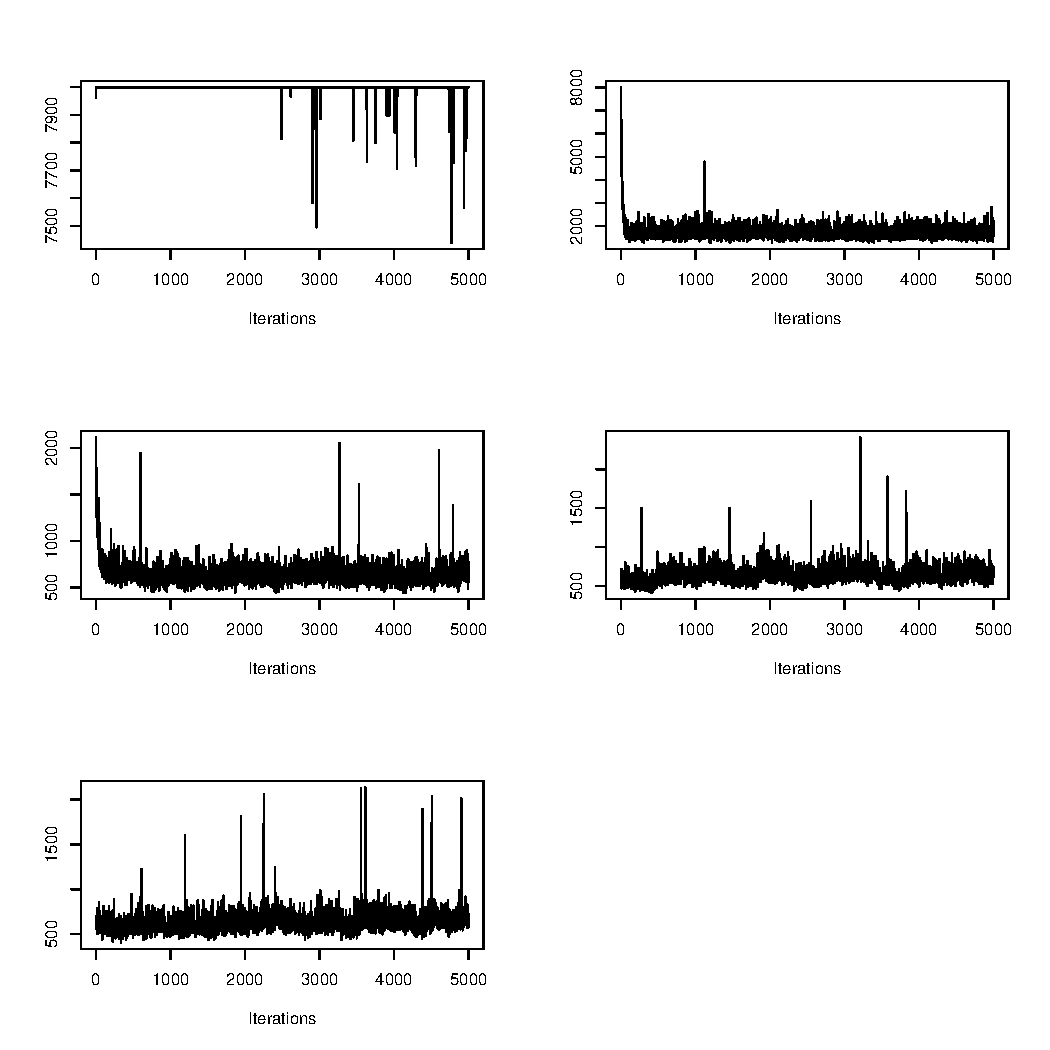
\includegraphics[height=.4\textheight]{5-cycles-max-id}
% 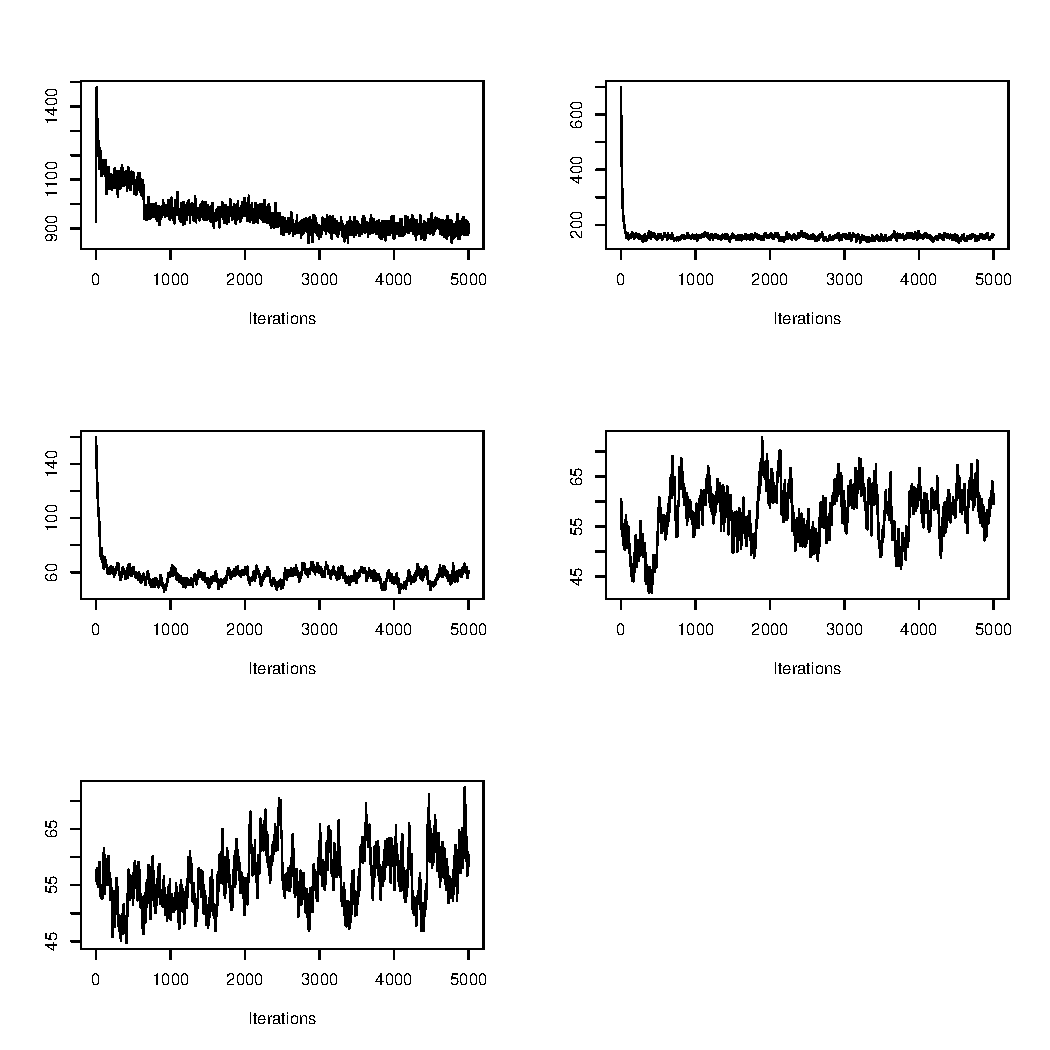
\includegraphics[height=.4\textheight]{5-cycles-alpha}
% \caption{Traceplots demonstrating high-level behavior after periodic reordering of cluster ids. Top: 5 series, maximum occupied cluster. Bottom: 5 series, $\alpha$.}
% \label{fig:max-id}
% \end{figure}


\subsection{Output}
\label{subsec:output}
Because of the dimensionality of the problem is large, it is cumbersome to save all of the MCMC samples. Following the approach in \citet{landau}, we preselect a small number of parameters for which we do save each iteration, but for the rest we first determine which functions of those parameters are of interest and use online algorithms that use running sums to update our estimates of those functions. The class of estimates we calculate fall into two categories,
\begin{enumerate}
\item expectations of the gene-specific parameters and their squares, i.e. $\op{E} \beta_g,\, \op{E} \beta_g^2,\, \op{E}\sigma_g,\, \op{E}\sigma_g^2$ and 
\item gene-specific posterior probabilities of conjunctions of linear
  inequalities of the elements of $\beta_g$, i.e.,
  $\op{Pr}\left(c_1\beta_g > 0 \land \ldots \land c_t\beta_g > 0\right)$.
\end{enumerate}
Updates of these quantities are embarrasingly parallel across $g$, so are well suited to the GPU. The update in 1) is done elementwise, based on a running sum, and the update in 2) can be decomposed into four tasks, a matrix multiplication to compute $C\beta$, an elementwise evaluation of the sign of the value, a parallel setwise reduction using the minimum to evaluate each conjunction, and finally an update of the estimator (using the same functionality as 1)).

We do save and return several low-dimensional parameters which provide some information on the overall behavior of the sampler: the number of occupied clusters, the maximum id of the occupied clusters and $\alpha$, the concentration parameter.


\section{Simulation Study}
\label{sec:timing}
To study the performance, we conducted a simulation study. To assess the time requirements, because time efficiency will depend both on the algorithmic implementation, that is, the raw time it takes to complete an MCMC iteration, but also on the statistical efficiency, i.e. the rate of mixing and the autocorrelation of the chain. Because it accounts for both factors, the measure we focus on is the time per effective sample. In particular, we focus on the samping for $\alpha$, both for simplicity and because it tends to reflect changes in the overall behavior of the Gibbs sampler.

We work with simulated data and consider three factors: $G$, the number of genes, $K$, the truncation limit, and $p$, the dimension of $\beta_g$. For each combination of the levels of these three factors we simulated data as shown below.

\paragraph{Cluster parameters}
Let $K_{t} = \op{floor}(G^{0.5})$. For $k=1 \ldots K_{t}$, draw $\tilde{\beta}_k \sim \op{Normal}(0, C),\; \tilde{\sigma^2}_k \sim \op{Gamma}(1, 1)$, where $C=\op{diag}(3, 3/2^2, \ldots, 3/p^2)$.
  
\paragraph{Allocation to clusters} For $g=1,\ldots G$, draw $\zeta_g \sim \op{Categorical}(1/K_{occ},\ldots,1/K_{occ})$. 
  
\paragraph{Conditionally normal data}
 Let $X = \begin{pmatrix} 1_{4 \times 1} & 0_{1\times(p-1)}\\
                                 1_{4(p-1) \times 1} & I_{(p-1)\times(p-1)} \otimes 1_{4\times 1} \end{pmatrix}$, where $\otimes$ is the Kronecker product. Draw $y_{g} \sim \op{Normal}(X\tilde{\beta}_{\zeta_g}, \tilde{\sigma}^2_{\zeta_g}).$


In this experiment we set the prior to the true values for $m_\beta = m$, and $C_\beta = C$ and set $a_\sigma^2=1$ and $b_\sigma^2=1$. Note that the true values $\sigma^2_k$ come from a gamma distribution, rather than an inverse gamma, which would have lead to dispropotionately high error variances for some genes. The prior for $\alpha$ is the one described in section \ref{sec:model}, with the prior expectation close or equal to the true value.

Results of the simulation study are presented in Table \ref{tab:neff-alpha}.

% latex table generated in R 3.4.1 by xtable 1.8-2 package
% Mon Aug 28 15:21:01 2017
\begin{table}[ht]
\caption{Number of seconds per effective sample for $\alpha$. Each value is computed from a 50,000 MCMC iterations (a single chain).}
\label{tab:neff-alpha}
\centering
\begin{tabular}{rrrrrr}

  &   & \multicolumn{3}{c}{K}\\
  \hline
G & p & 1024 & 2048 & 4096 \\ 
  \hline
4096  & 2 & 17 & 30 & 241 \\ 
      & 4 & 9 & 8 & 127 \\ 
      & 6 & 3 & 4 & 140 \\ 
8192  & 2 & 28 & 40 & 231 \\ 
      & 4 & 11 & 19 & 111 \\ 
      & 6 & 7 & 21 & 35 \\ 
16384 & 2 & 25 & 56 & 167 \\ 
      & 4 & 13 & 25 & 150 \\ 
      & 6 & 8 & 17 &  \\ 
32768 & 2 & 66 & 101 & 267 \\ 
      & 4 & 6 & 46 & 113 \\ 
      & 6 & 12 & 31 & 108 \\ 
   \hline
\end{tabular}

\end{table}

% \begin{figure}
% \centering
% 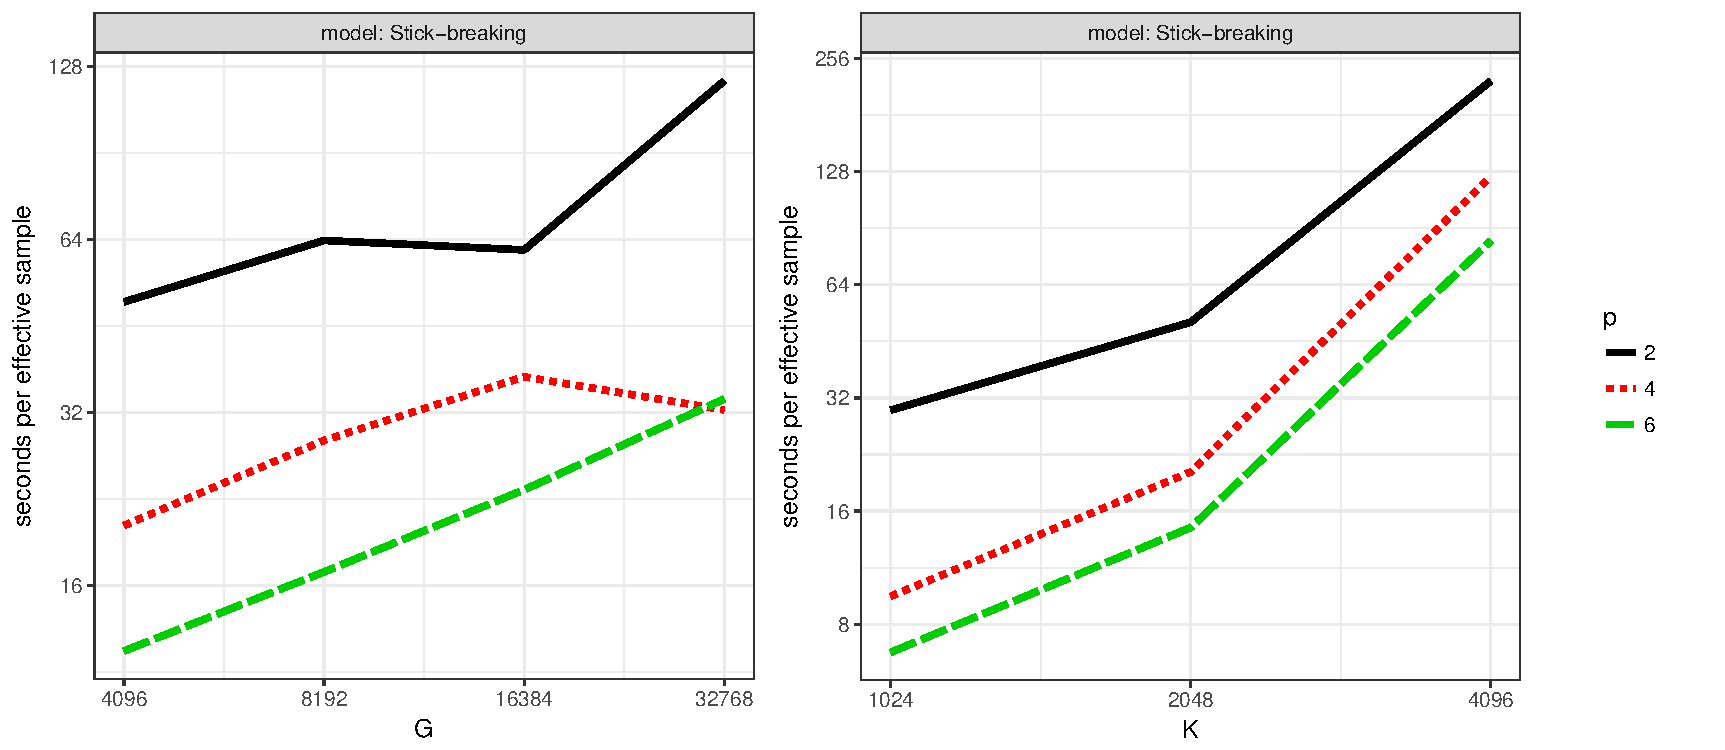
\includegraphics[width=.9\textwidth]{neff-marginal}
% \caption{Number of effective samples for $\alpha$ marginalizing over the third factor (left:K, right:G).}
% \label{fig:neff-marginal}
% \end{figure}

\begin{figure}[ht]
\centering
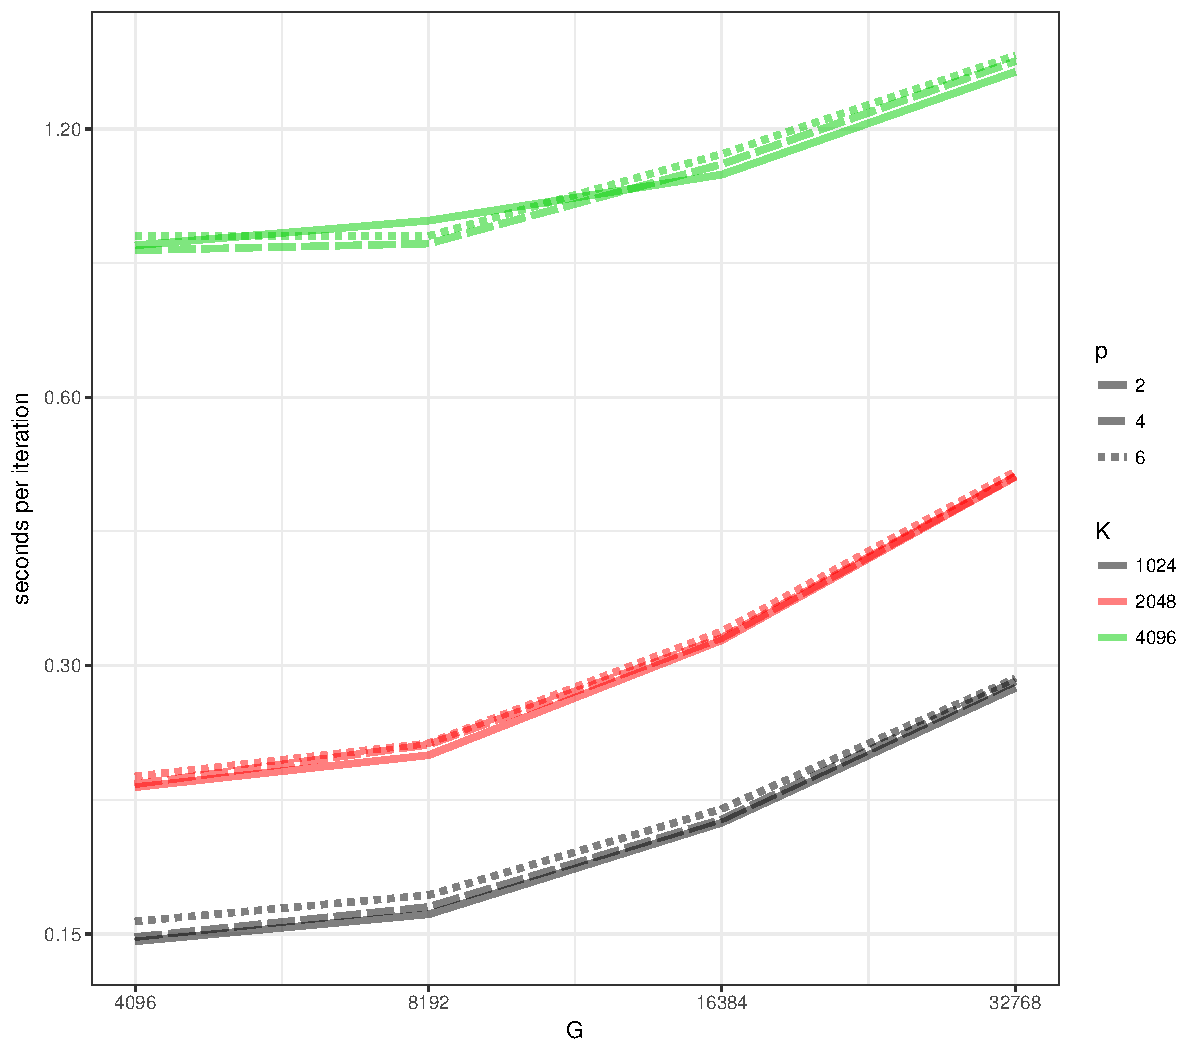
\includegraphics[width=.9\textwidth]{raw-time2}
\caption[Average number of seconds per MCMC sample]{Left: Average seconds required per MCMC sample across for two simulated datasets at each level of K, the truncation limit, G, then number of genes, and p , the dimension of regression coefficient. K has the largest impact on computation time, followed by G. The effect of p is small in the range considered. For large K and small G, the cost of increasing p appears to be offset by the smaller number of occupied clusters in a higher dimensional space.}%
\label{raw-time}
\end{figure}

\begin{figure}[ht]
\centering
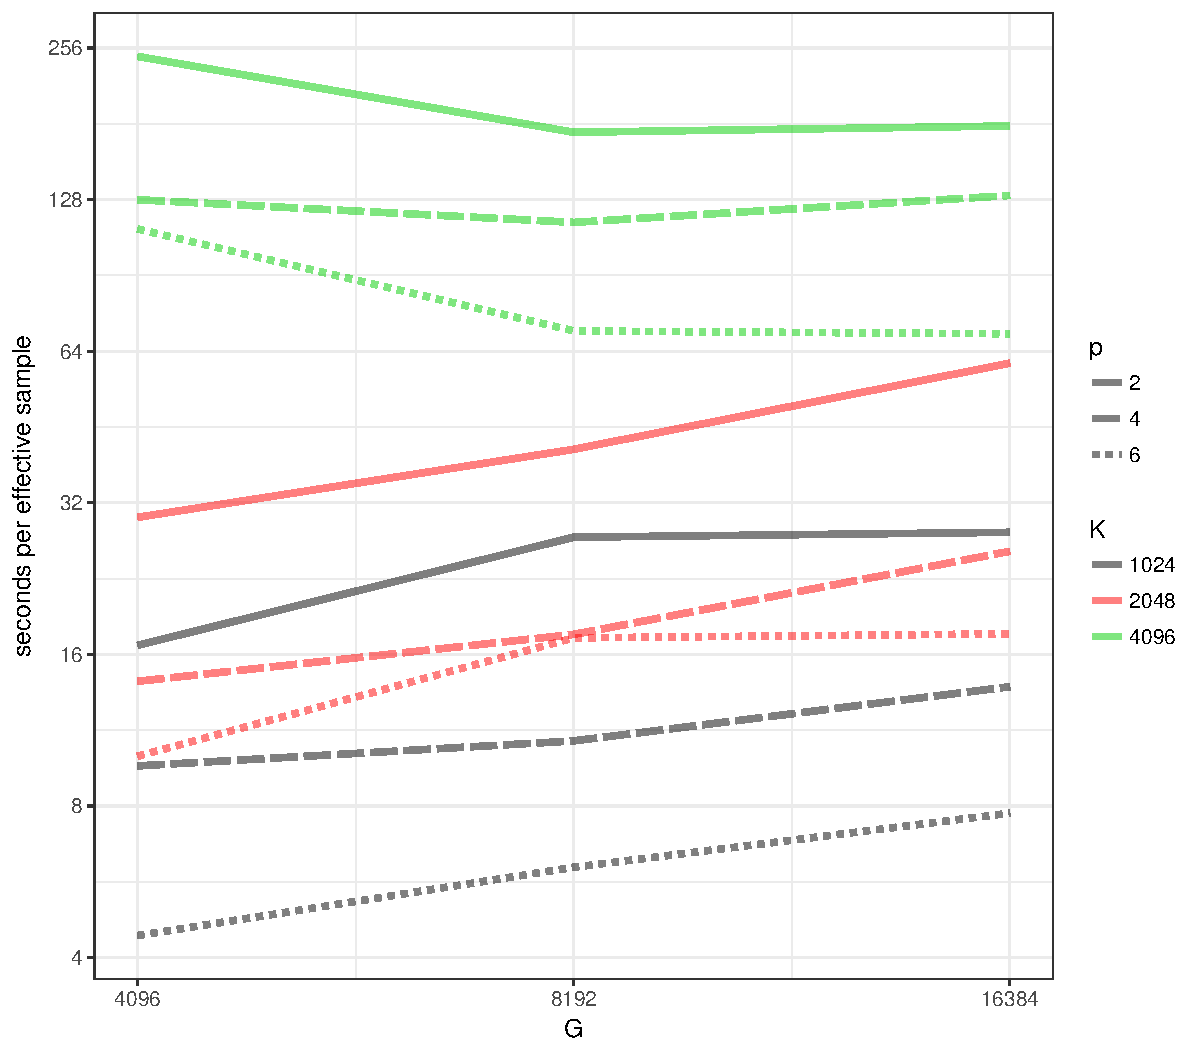
\includegraphics[width=.9\textwidth]{eff-time2}
\caption[Average seconds per effective sample]{Left: Average seconds per effective sample across for two simulated datasets at each level of K, the truncation limit, G, then number of genes, and p , the dimension of regression coefficient. Interestingly, the efficiency in sampling for $\alpha$ increases with p in our simulations. This might be explained by an increased separation between clusters, leading to greater stability in the partition defined by the allocation parameters.}%
\label{eff-time}
\end{figure}

% latex table generated in R 3.4.1 by xtable 1.8-2 package
% Wed Sep 06 08:56:57 2017
\begin{table}[ht]
\caption[Estimated exponentiated coefficients for the linear regression model: (model)]{Estimated exponentiatedcoefficients for the linear regression model: \\\hspace{\textwidth}\(\log_2$(sec. per eff. sample)$=\beta_0 + \log_2(K)\beta_1 + \log_2(G)\beta_2 + \log_2(V)\beta_3 + \epsilon\). The exponentiated values are a multiplicative effect on the predicted median seconds per effective sample for each doubling in the corresponding predictor (K,G or V).}
%   Estimated coefficients for the linear regression model,.}
\label{tab:regression}
\centering
\begin{tabular}{rrrr}
  \hline
 & Est. & lower 95\% & upper 95\% \\ 
  \hline
$2^{\beta_1}$ & 3.251 & 2.807 & 3.765 \\ 
  $2^{\beta_2}$ & 1.171 & 1.011 & 1.357 \\ 
  $2^{\beta_3}$ & 0.485 & 0.404 & 0.582 \\ 
   \hline
\end{tabular}
\end{table}

Table \ref{tab:regression} shows the result of fitting a linear regression of $\log_2(\frac{\mbox{seconds}}{\mbox{effective sample}}$ on $\log_2(K)$, $\log_2(G)$ and $V$. The estimated coefficients of this additive model suggest that seconds per effective sample grows sublinearly in $G$, approximately quadratic in $K$ and inversely with $V$.

\iftoggle{thesis}{
  This last observation may seem counterintutive; however, because the posterior variability of $\alpha$ depends on the stability of the the partition of genes into clusters, and as $p$ increases so does the distance between clusters, $\alpha$, like the partition, has fewer viable moves. This phenomenon is also on display in Figure \ref{alpha-trace} where the normalized traceplots seem to show shorter and less extreme excursions in the higher dimensions.
  
  \begin{figure}[ht]
  \centering
  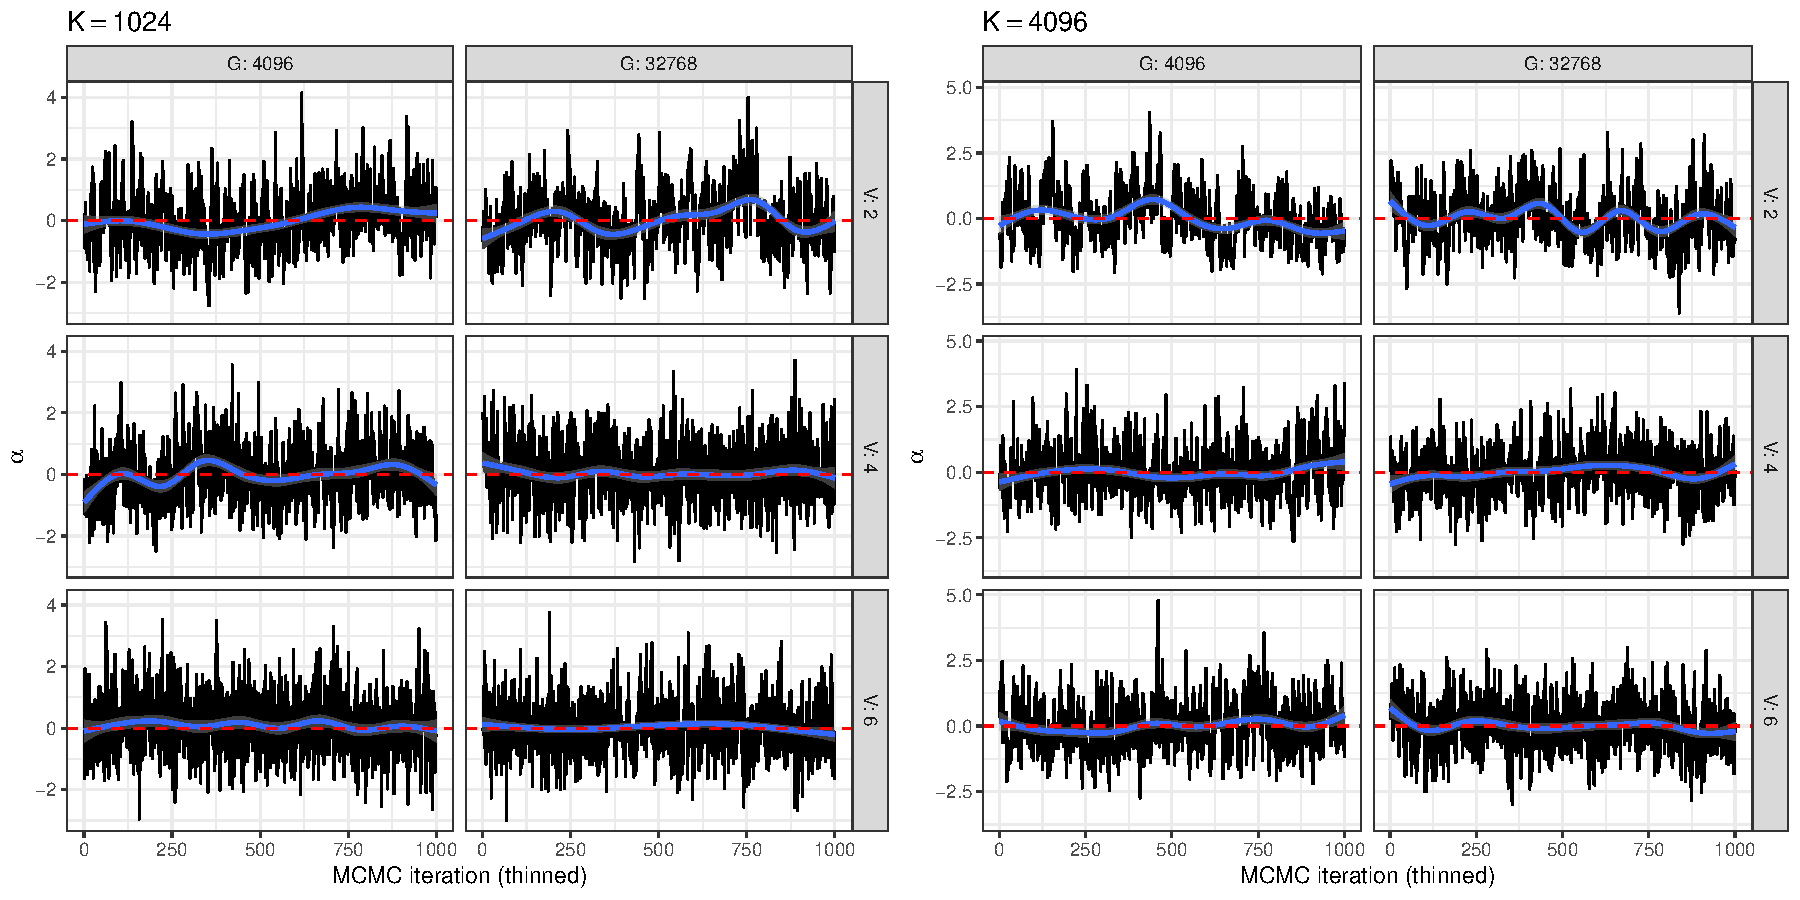
\includegraphics[width=.9\textwidth]{alpha-efficiency}
  \caption{Centered and scaled traceplots for $\alpha$ across levels of $p$ for various settings of $G$ and $K$.}
  \label{alpha-trace}
  \end{figure}
}

\section{Example: Paschold maize data}
\label{sec:analysis}
\citet{paschold} produced an RNA-seq data set for gene expression of root tissue from 4 samples for each of two recombinant inbred maize genotypes, B73 and Mo17. Each sample was obtained from a combination of 10 primary roots from seedlings 3.5 days after germination. Illumina's Genome Analyzer II was used for sequencing. Two flow cells were utilized, with four replicates of each genotype split across flowcells. Among the researchers' aims was to identify genes which were differentially expressed in these parental lines.

\subsection{Model}
We let $Y_{gci} = \log \frac{Z_{gci}+1}{C_{ci}}$, where $Z_{gi}$ is the total read count for replicate $i$ of genotype $c$. $C_{ci}$ is a normalizing constant which is used to adjust for differences in the total RNA content in each sample. We estimate the normalizing constants using the trimmed mean of M-values procedure \cite{robinson2010}. Our design matrix for each gene (collapsing identical rows) is

\begin{equation*}
\begin{blockarray}{rlrrr}
  && \mbox{(intercept) }\beta_1 & \mbox{(Mo17) }\beta_2 & \mbox{(flow cell) }\beta_3\\
  \begin{block}{rl(rrr)}
  \mbox{B73}    &\mbox{reps:1,2} & 1 & 0 & 0\\
  \mbox{B73}    &\mbox{reps:3,4} & 1 & 0 & 1\\
  \mbox{Mo17}   &\mbox{reps:1,2} & 1 & 1 & 0\\
  \mbox{Mo17}   &\mbox{reps:3,4} & 1 & 1 & 1\\
  \end{block}
\end{blockarray}
\label{design}
\end{equation*}

We fit the model using four independent chains. They were initialized by setting unique random seeds and running 1000 iterations, then reordering the cluster indices by $\pi$. 50,000 iterations were run for each chain after 10,000 iterations of burn-in. Potential scale reduction factors are shown in figure \ref{rhat}. Values close to 1 are consistent with convergence; 1.1 has been suggested as a cut-off. While some parameters exceeded 1.1, the vast majority were close to 1.

\begin{figure}
\centering
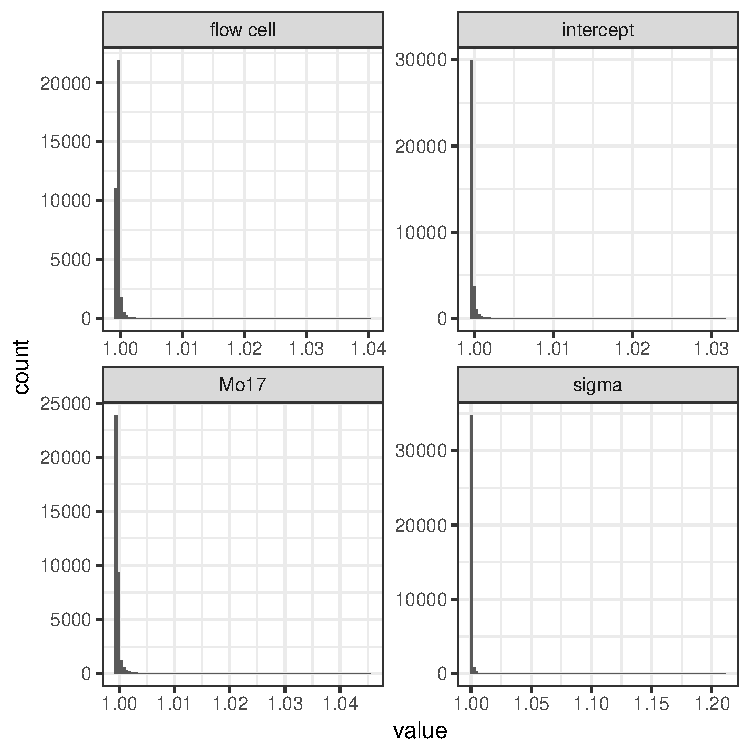
\includegraphics[width=.8\textwidth]{rhats-param}
\caption{Gelman-Rubin potential scale reduction factors for all gene-specific parameters.}
\label{rhat}
\end{figure}

\subsection{Comparison of methods}
In addition to our method, we also fit the data using two other model: a linear mixed-effects model, treating gene-specific parameters as random effects, and all genes independently using least squares. For every method we parameterized the gene-specific mean with an intercept, an additive effect for the $Mo17$ genotype, and an additive effect for flow cell 2. The gene independent model, which produces a gene-specific variance estimate borrows no information across genes. The linear mixed-effects model assumes a bivariate normal distribution for all the gene-specific mean parameters. Because the covariance and the mean of this distribution is estimatated from the data, this model does borrow information across genes (since software assumes a zero mean for the random gene effects, we also estimate a fixed effect which corresponds to the unknown mean.) This method assumes homogeneity of the error variance across genes.

\begin{figure}
\centering
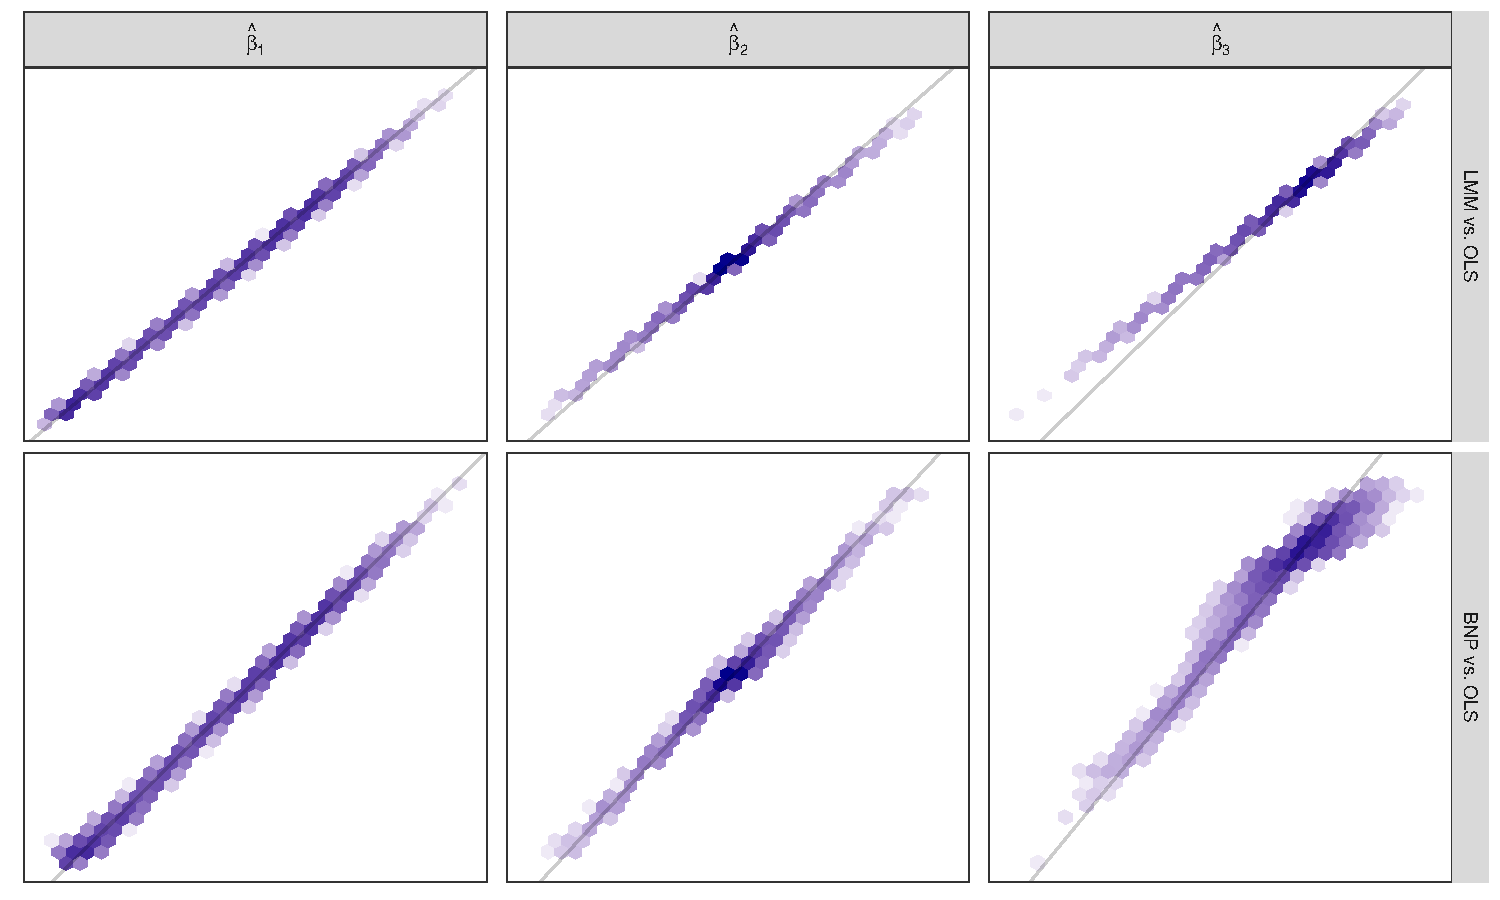
\includegraphics[width=.9\textwidth]{method-compare-std}
\caption{Comparisons of the parameter estimates under each method.}
\label{method-compare}
\end{figure}
Figure  \ref{method-compare} shows a comparison of the estimates under three models. While there is agreement about the gene-specific intercepts, there is noticable shrinkage toward the global mean for the half-difference in the linear mixed-effects model. This can be explained by the long tail of these estimates relative to a normal distribution.

Figures \ref{pairs-3-methods} and \ref{diff-hist} show slices in two dimensions of the joint distribution of point estimates provided by the three models, and differences of these empirical densities. Figure \ref{diff-hist} reveals a key distinction between BNP and LMM, that the shrinkage under LMM is monotonic toward a single point, whereas BNP shrinks estimates in different ways depending on their general location in the parameter space. This is most clearly illustrated by the third row, which compares the bivariate densities of point estimates of $(\beta_{g2},\beta_{g3})$ under the different models. The estimates obtained by BNP are shrunken toward two perpendicular line segments which follow the center of the distribution of the OLS estimates. The normality assumption of LMM leads to the points along the vertical axis being all shrunk monotonically toward the origin. The bottom-left plot in figure \ref{diff-hist} shows that estimates of $\sigma_g$ are clearly shrunken toward a curve which can be interpreted as an estimate of a latent mean-variance trend across genes. This is significant, as compensating for such a trend is a recognized objective in the analysis of RNA-seq data.

\begin{figure}[ht]
\centering
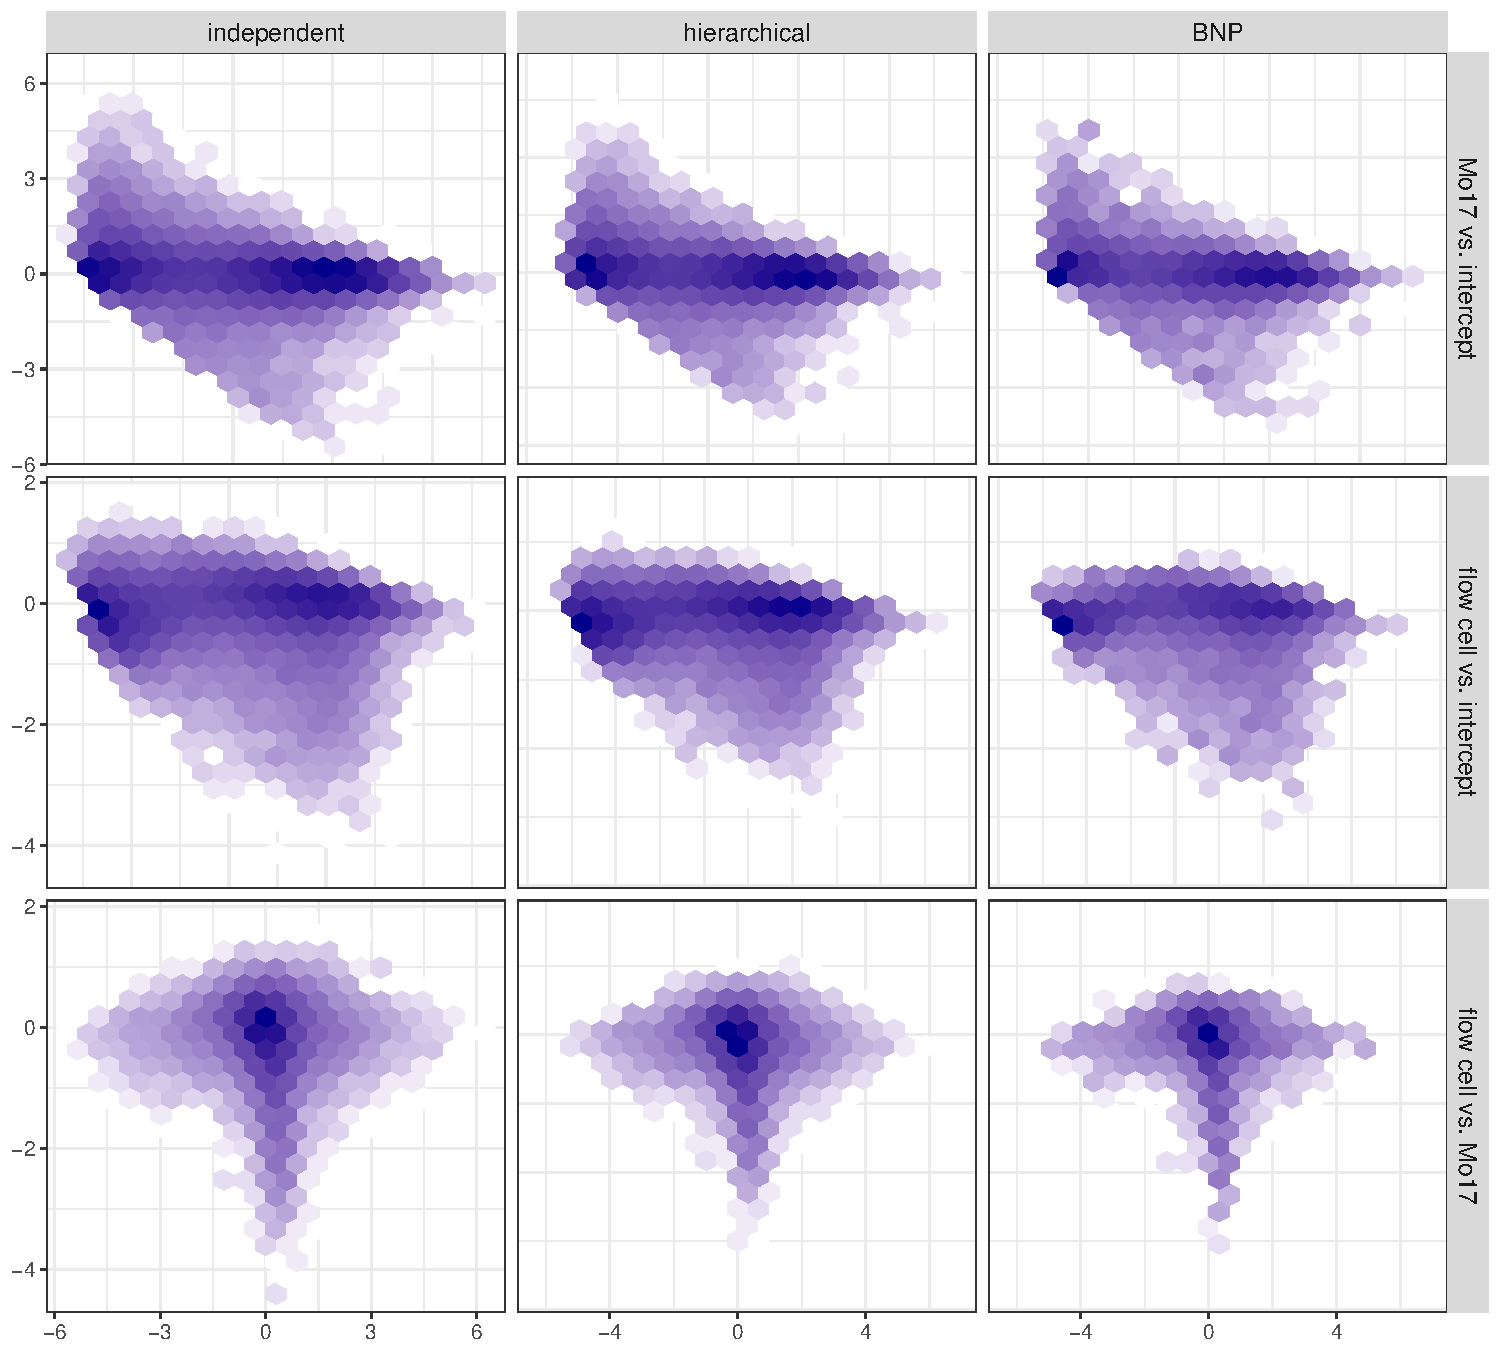
\includegraphics[width=.9\textwidth]{pairs-3-methods-std}
\caption{Histogram of point estimates across genes, showing pairwise comparisons, using hexagonal binning. Relative to the independent estimates obtained by least-squares ("OLS"), the linear mixed-effects model ("LMM") shrinks all estimates toward a common mean, while the Bayesian nonparametric model shrinks estimates toward an underlying distribution learned from the data.}
\label{pairs-3-methods}
\end{figure}

Figure \ref{pairs-3-methods} displays pairs of parameter estimates obtained from the different methods. The top two rows shows slight differences in the joint distribution of the gene-specific mean parameters for OLS when compared with those obtained by LMM. This difference is characterized by a shrinkage of all estimates toward the overall average, which has most noticable impact on the genes which are estimated to be far from that average.

\begin{figure}[ht]
\centering
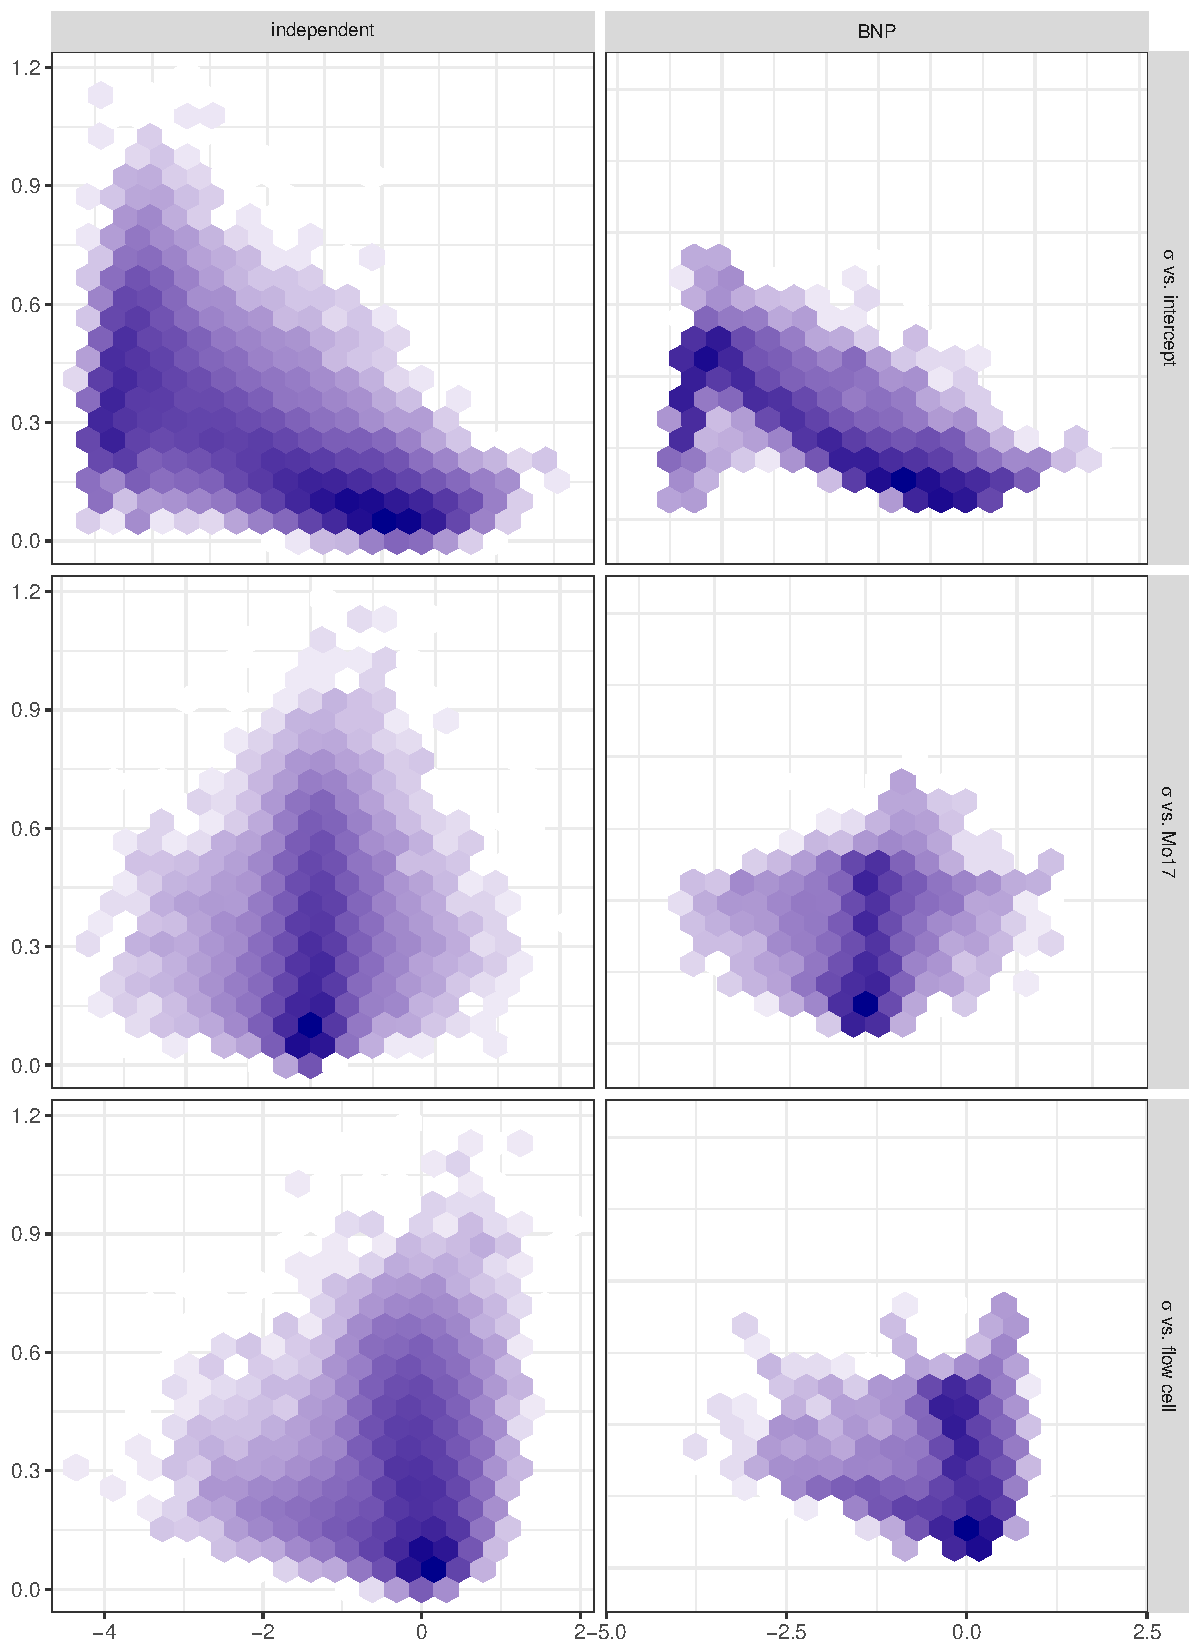
\includegraphics[width=.65\textwidth]{mean-variance}
\caption{Bivariate histogram of point estimates across genes, using hexagonal binning. Relative to the independent estimates obtained by least-squares ("OLS"), the Bayesian nonparametric model shrinks estimates toward an underlying distribution learned from the data.}
\label{mean-variance}
\end{figure}

\begin{figure}[ht]
\centering
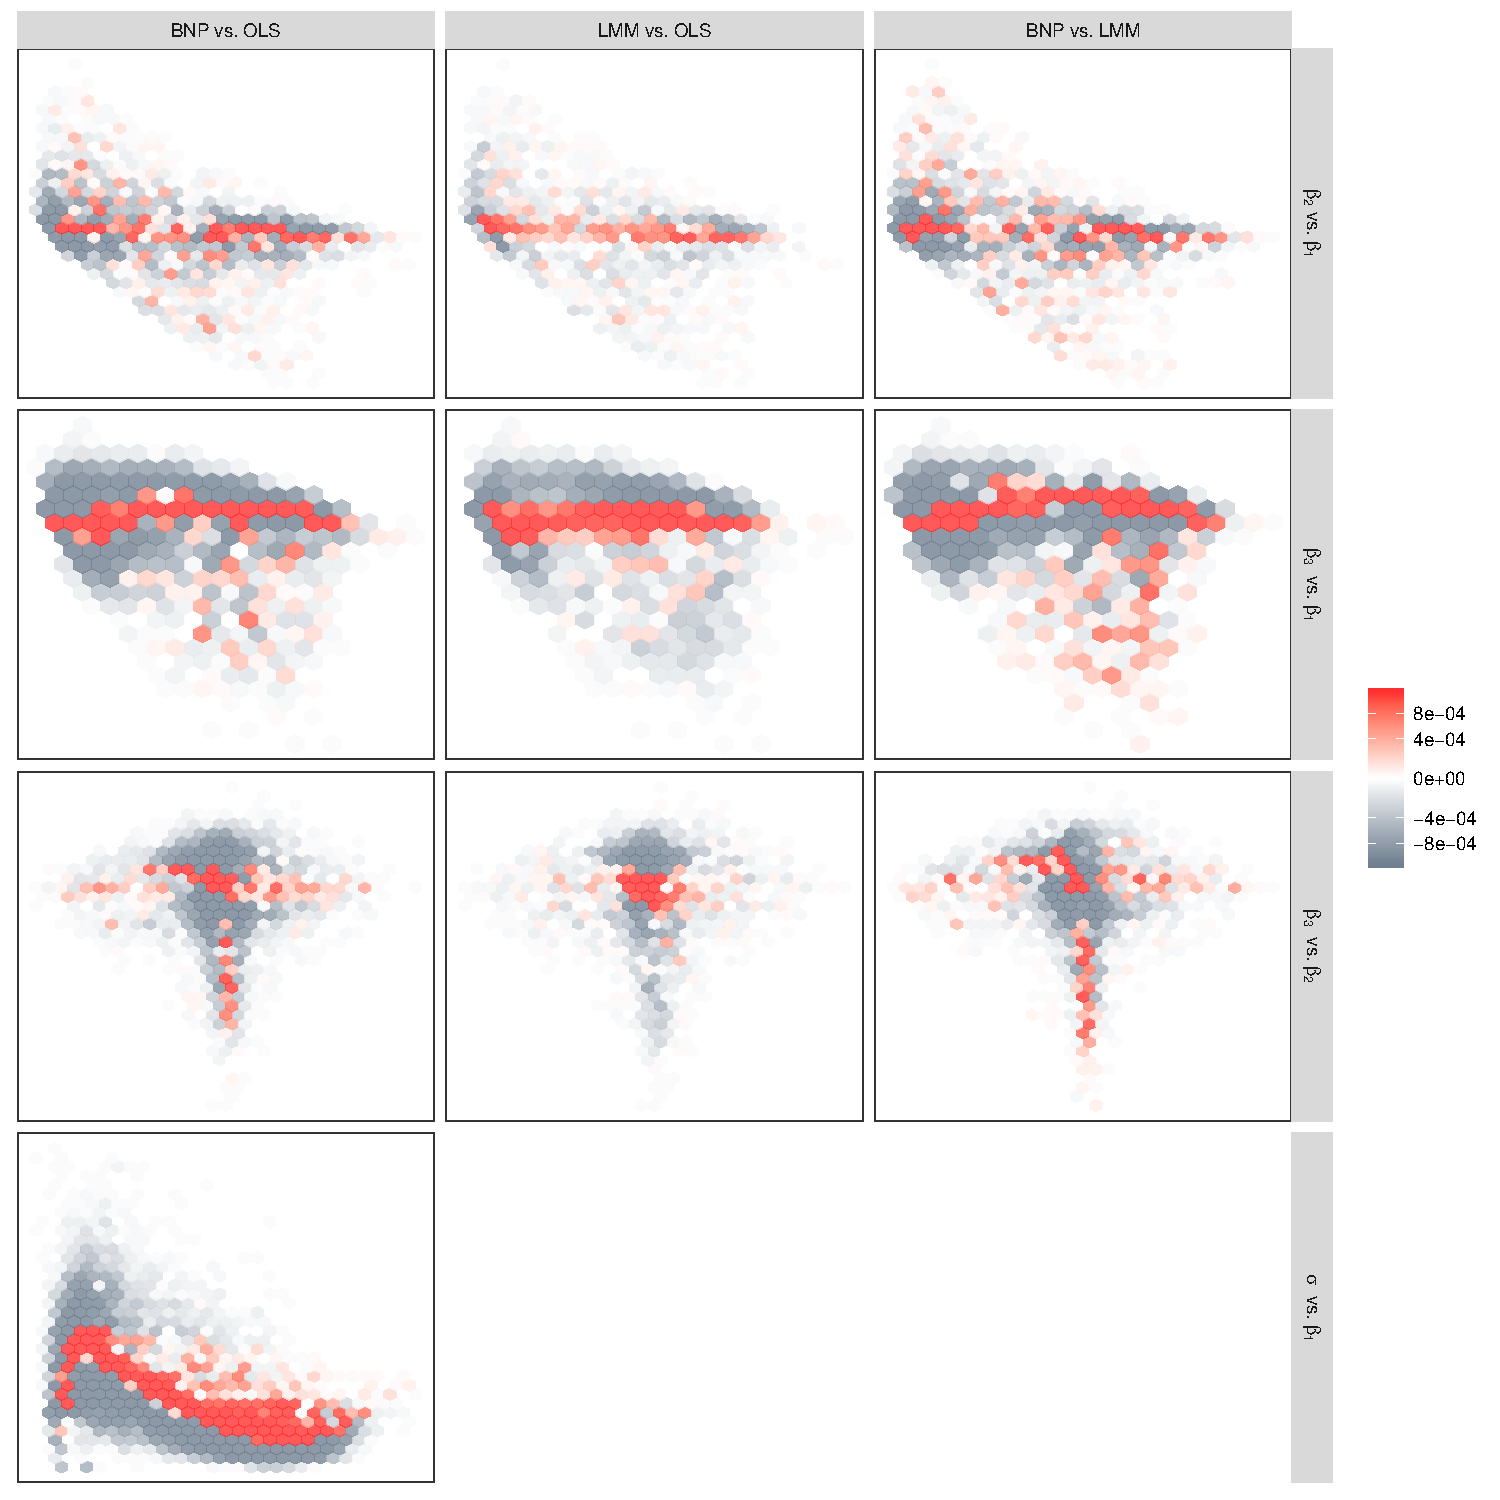
\includegraphics[width=\textwidth]{difference_histograms}
\caption{Difference of histograms of point estimates for gene-specific parameters under different models. Both BNP and LMM show shrinkage toward zero relative to OLS. The shrinkage with LMM is monotonic toward zero, while the shrinkage with BNP varies across the parameter space.}
\label{diff-hist}
\end{figure}


% Of particular interest was the identification of genes where the mean hybrid expression is higher or lower than that of both parents. For each gene, a reduced version of the design matrix (collapsing identical rows) is
% \begin{equation*}
% \begin{blockarray}{lcccc}
%   & \beta_1 & \beta_2 & \beta_3 & \beta_4\\
%   \begin{block}{l(cccc)}
%   \mbox{B73} & 1 & 1 & 0 & 0\\
%   \mbox{Mo17} & 1 & -1 & 0 & 0\\
%   \mbox{B73$\times$Mo17} & 1 & 0 & 1 & 1\\
%   \mbox{Mo17$\times$B73} & 1 & 0 & 1 & -1\\
%   \end{block}
% \end{blockarray}
% \label{design}
% \end{equation*}
% 
% In figure \ref{ggpairs_us}, histograms of the empirical distributions of the OLS estimates are shown. The irregularities seen here contraindicate the use of simple independent parametric models for the underlying parameters. In particular, we note the multimodality of $\beta_1$, the rotated `V' shape of $(\beta_2,\beta_3)$. Despite a large number of genes, we suspect that a misspecification of the model for these parameters will limit the efficacy of borrowing information across genes. We seek to improve the efficacy of borrowing information by relaxing the model to allow Bayesian learning about the underlying distribution of these parameters.
% \begin{figure}
% 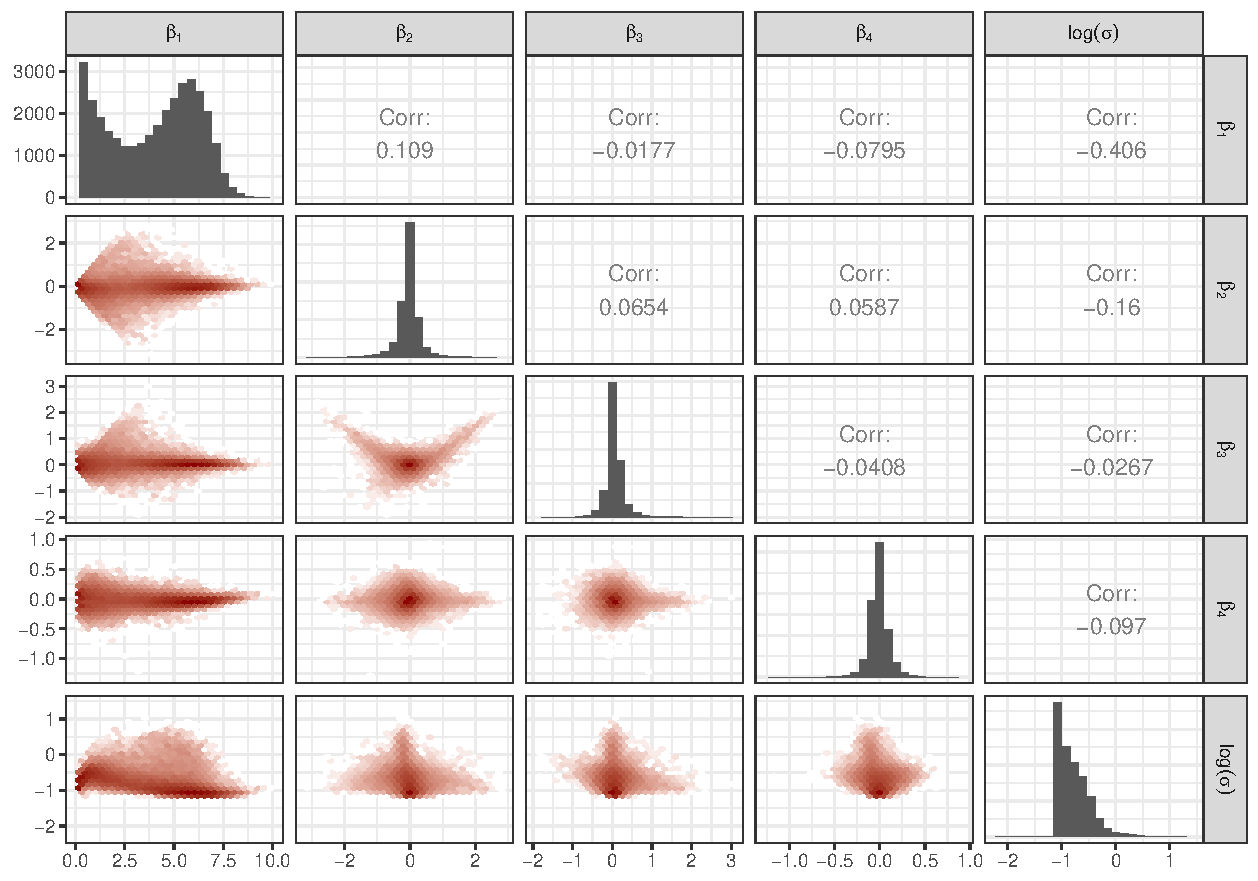
\includegraphics[width=\textwidth]{ggpairs_us}
% \caption{Histograms and pairwise histograms of independent OLS
%   estimates to for $(\beta_g,\log \sigma_g)$ for all genes in Paschold data set with a non-zero count.}
% \label{ggpairs_us}
% \end{figure}
% 
% Estimates of the posterior means after fitting our model are shown in figure \ref{ggpairs_s}.
% \begin{figure}
% 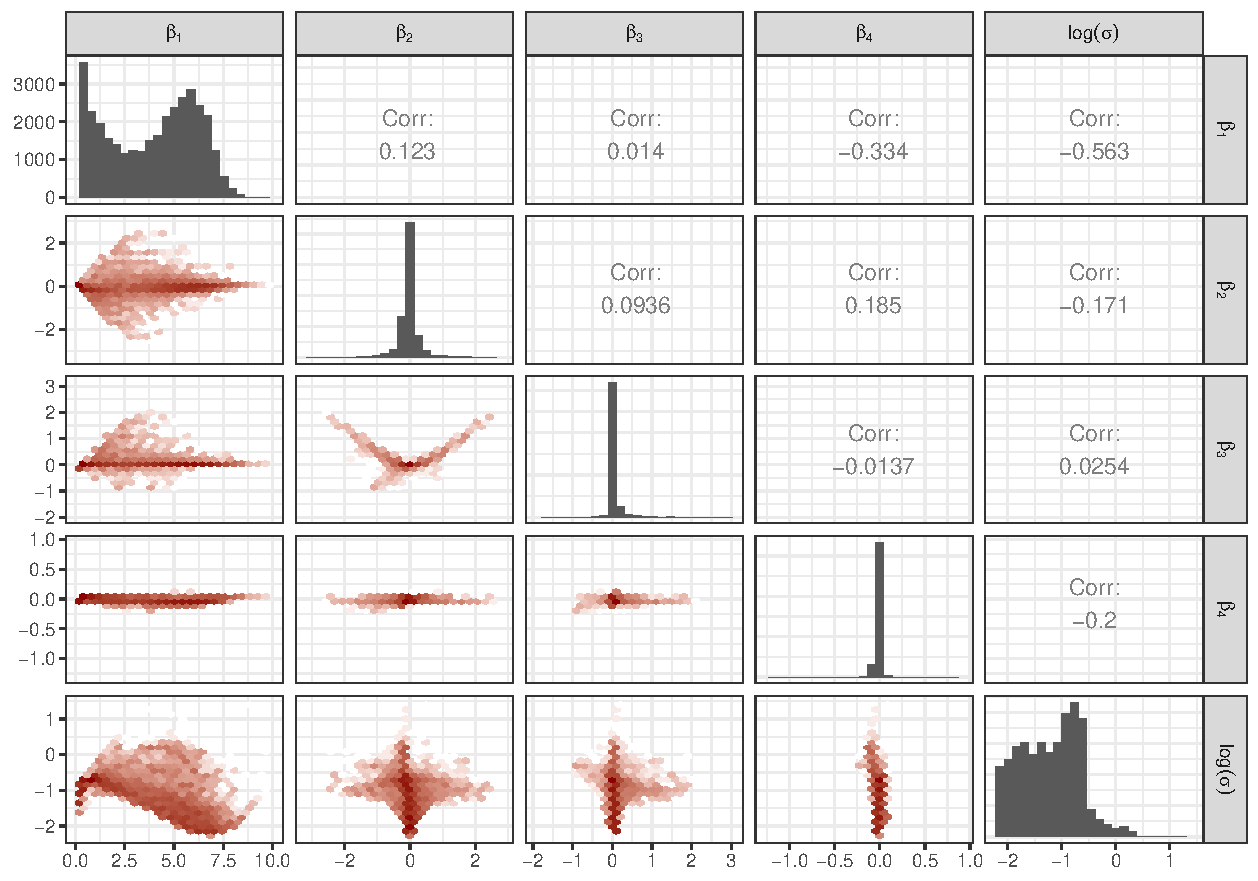
\includegraphics[width=\textwidth]{ggpairs_s}
% \caption{Histograms and pairwise histograms of posterior means of
%   nonparametric model. Relative to the estimates in Figure
%   \ref{ggpairs_us}, there is substantial shrinkage acheived by latent
%   clustering.}
% \label{ggpairs_s}
% \end{figure}

\section{Discussion}
\label{sec:discussion}
Although quite computationally intensive, nonparametric Bayesian methods are becoming computationally feasible in applications, even for fairly sizable datasets, such as gene expression profiling. One way to achieve computational feasibility is through adapting existing procedures to take advantage of massively parallel systems like the GPU.

We have found some evidence that our proposed procedure scales well with the size of the data ($G$), as well as the dimension of the problem ($V$), and is approximately quadratic in the number of clusters required to approximate the latent infinite mixture ($K$).

\appendix
\section{CUDA libraries}
There are several libraries that make implementing these algorithms easier in CUDA. Thrust \citep{thrust} extends many concepts from the C++ Standard Template Library to Nvidia GPUs. Included are several useful generic algorithms:
\begin{itemize}
\item \code{thrust::for\_each}: This algorithm accepts a functor (an
  instance of a class with a member \code{operator()} function)
  and an iterator. The serial version increments the iterator, passing
  each element to the \code{operator()} in turn. The parallel implementation
  produces the same results, only in thread parallel fashion. The
  \code{thrust::zip\_iterator} is very useful, as it can be used
  to iterate
  over a \code{thrust::tuple}. This approach is very general, allowing
  for operations involving up to ten variables using an AoS
  design.

\item \code{thrust::reduce/reduce\_by\_key}: As described in section
  \ref{sec:parallel}, both reduce and cumulative sum are defined for any associative binary operators. Reduce by key accepts a key argument and a compatible binary predicate that identifies changes in the key. For example, for the binary predicate \code{x == y}, the key \code{\{1,1,1,2,2,1\}} would have the result be three quantities, the reductions of the first three values, the next two and the last, respectively.

\item \code{thrust::inclusive/exclusive\_scan/scan\_by\_key}: Thrust
  offers multiple versions of scan, which is another term for cumulative sum. The exclusive
  version results in the array element, $a_i$, containing the sum $s_{i-1}$ (excluding the value $v_i$, while the inclusive version leaves $a_i$ containing $s_i$.
\end{itemize}

For linear algebra on the GPU, standard installations of CUDA also
include CUBLAS \cite{cublas}. CUBLAS has implementions of BLAS/LAPACK
routines optimized for the GPU. Typically, calls to the CUBLAS
functions are initiated by the CPU and act on device memory (host
API). For newer GPUs (compute 3.5 and later), there are routines that
can be initiated within a kernel (device API). From the host API, our
algorithm uses \code{cublasDgemm} for multiplying large matrices in
device memory. From the
device API, our algorithm uses \code{cublasDtrsv} to solve many small triangular
systems of equations in parallel.

Schemes for parallel pseudo-random number generation (PRNG) have been
developed for CUDA. Since PRNGs are deterministic and sequential, a
natural parallel adaptation is access the same sequence at locations
distant enough to avoid overlap or to use a strided access
pattern. CURAND \cite{curand}, provides such functionality for generating
normal and uniform random numbers on the GPU. For other distributions,
such as gamma,
one can write a custom kernel, making use of CURAND as a source of
randomness, for threaded sampler.



  
  \bigskip
  \begin{center}
  {\large\bf SUPPLEMENTAL MATERIALS}
  \end{center}
  
  \begin{description}
  
  \item[Title:] Brief description. (file type)
  
  \item[R-package for  MYNEW routine:] R-package ÒMYNEWÓ containing code to perform the diagnostic methods described in the article. The package also contains all datasets used as examples in the article. (GNU zipped tar file)
  
  \item[HIV data set:] Data set used in the illustration of MYNEW method in Section~ 3.2. (.txt file)
  
  \end{description}
  
  \appendix
  \include{appendix}
  
  \bibliographystyle{apalike}
  \bibliography{computation}
  
  \end{document} 